%%%%%%%%%%%%%%%%%%%%%%%%%%%%%%%%%%%%%%%%%%%%%%%%%
%%%
%%% Auteur : Stéphane Péchard - stephane.pechard@univ-nantes.fr
%%% Fichier : 7-modClassif.tex - chapitre 7 : Exploitation de la segmentation spatio-temporelle dans des critères objectifs de qualité vidéo
%%% Version : 0.1
%%% Date :	2007/11/26
%%%
%%%%%%%%%%%%%%%%%%%%%%%%%%%%%%%%%%%%%%%%%%%%%%%%%
\chapter{Exploitation de la segmentation spatio-temporelle dans des critères objectifs de qualité vidéo} \label{chap:modeleDistorsionsTubes}
\opt{final}{\lettrine[lines=4]{L}{e chapitre précédent a montré}}\opt{nofinal}{Le chapitre précédent a montré} qu'il était possible de créer un critère de qualité vidéo performant adapté à la télévision haute définition dans un contexte de codage. Dans ce dernier chapitre, nous cherchons à exploiter le résultat de la segmentation spatio-temporelle présentée au chapitre~\ref{chap:methode}. Pour cela, nous proposons deux approches différentes. La première estime les pertes locales de qualité et utilise les fonctions de cumul présentées à la section~\ref{sec:deLocalAGlobal} pour produire une note de qualité. La seconde approche cherche plus particulièrement à qualifier et valider l'apport de l'utilisation des zones spatio-temporelles élémentaires orientées selon le mouvement. Dans le chapitre~\ref{chap:MQV1}, nous utilisions uniquement les proportions de chaque classe de contenu issues de la classification. Ici, nous exploitons les tubes spatio-temporels afin de construire un critère objectif de qualité avec référence complète basé sur une mesure de caractéristiques primaires dans ces tubes. Les écarts entre caractéristiques mesurées dans les tubes de la séquence de référence et celles mesurées dans la séquence dégradée nous conduit à prédire la qualité de la séquence dégradée. Nous comparerons les performances obtenues par ce critère avec celles obtenues par les critères VSSIM et VQM. Une version simplifiée de notre approche sera également développée, ne prenant pas en compte le mouvement.


\section{Approche fondée sur des modèles de perte de qualité}
Dans ses travaux, Farias~\cite{farias-phd} propose une fonction de gêne par type de dégradation. Étant donné qu'elle génère ses dégradations de manière synthétique, elle en contrôle parfaitement l'intensité. Pour chacune d'entre elles, elle dispose d'un paramètre relié à celle-ci, comme par exemple la taille du filtre pour l'obtention du flou. La gêne qu'elle mesure est donc fonction de ces paramètres. Cependant, dans notre méthodologie présentée au chapitre~\ref{chap:methode}, nous n'avons pas de contrôle aussi précis sur l'injection de dégradations dues au codage \avc{} dans une classe de contenu donnée. En effet, le débit total est alloué pour tout le domaine spatio-temporel de la séquence et nous n'avons pas un accès assez fin à la manière dont il le répartit localement. Éventuellement, le codeur fournit des informations synthétiques sur le codage image par image. Cela peut renseigner sur la répartition temporelle, mais pas spatiale.

La figure~\ref{fig:chap7Approche1} présente le fonctionnement de cette première approche. Notre technique de segmentation spatio-temporelle permet de connaitre les proportions et les vecteurs de mouvement des classes de contenu. Ajoutés à une mesure d'erreur entre la séquence dégradée et la séquence de référence, ces informations permettent la construction d'un paramètre de contrôle de la quantité de dégradations présentes dans une classe. À partir de ce paramètre, une modélisation de la perte de qualité permet d'obtenir une fonction de gêne par classe. Enfin, une fonction de cumul, comme celles présentées à la section~\ref{sec:deLocalAGlobal}, produit une note finale de qualité. Dans un premier temps, nous cherchons à identifier les facteurs impliqués dans la perte de qualité dans les classes, afin de construire un paramètre de distorsion. %Une fois à notre disposition, un tel paramètre peut ensuite être utilisé dans la construction d'un modèle de perte de qualité. Nous présenterons un tel modèle pour la classe $C_1$ des zones homogènes de faible luminance.

\begin{figure}[htbp]
	\centering
	\begin{tikzpicture}[text centered, node distance=2cm]% 	\begin{tikzpicture}[text centered, node distance=2cm] % , text width=2cm
		\node[text width=1.9cm] (ref) {séquence de référence};
		\node[right of = ref] (rightOfRef) {};
		\node[action, right of = rightOfRef, text width=2cm, node distance=0.5cm] (seg) {segmentation spatio-temporelle};
		\node[below of = seg, node distance=1.5cm] (belowOfSeg) {};
		\node[action, right of = belowOfSeg, node distance=3.2cm, text width=2cm] (cons) {construction d'un paramètre de contrôle de la quantité de dégradations d'une classe};
		\node[action, right of = cons, text width=1.5cm, node distance=2.4cm] (fGene) {fonction de gêne par classe};
		\node[action, right of = fGene, node distance=2.3cm, text width=1.9cm] (cumul) {cumul inter-classes des pertes de qualité};
		\node[right of = cumul, text width=1.5cm, node distance=2.3cm] (out) {note de qualité};

		\node[action, below of = ref, text width=1.3cm, node distance=3cm] (mse) {calcul d'erreur};
		\node[below of = mse, node distance=2cm, text width=1.5cm] (deg) {séquence dégradée};

		\draw[fleche] (ref) -- (mse);
		\draw[fleche] (deg) -- (mse);
		\draw[fleche] (ref) -- (seg);
		\draw[fleche] (seg) |- (cons) node[text width=3cm, pos=0.75] {vecteurs de mouvement};
		\draw[fleche] (seg) -- node[pos=1,above =0.3cm] {proportions} (cons.west |- seg);
		\draw[fleche] (mse) -- node[above] {erreur} (cons.west |- mse);
		\draw[fleche] (cons) -- (fGene);
		\draw[fleche] (fGene) -- (cumul);
		\draw[fleche] (cumul) -- (out);
% 	\end{tikzpicture}
\end{tikzpicture}
	\label{fig:chap7Approche1}
	\caption{Fonctionnement de l'approche fondée sur des modèles de perte de qualité.}
\end{figure}


\subsection{Facteurs de perte de qualité et contrôle de la quantité de dégradations}
Plusieurs facteurs sont à l'origine de la perte de qualité due au codage dans une même classe $C_i$. Le premier est bien sûr les dégradations en elles-mêmes, qui correspondent à une distorsion entre la vidéo originale et la vidéo dégradée. Par ailleurs, le mouvement apparent contribue aussi aux dégradations, d'autant plus que nous considérons des écrans de technologie LCD. Ensuite, chaque classe a sa propre proportion dans le domaine spatio-temporel des contenus. Celle-ci joue aussi un rôle dans la quantité de dégradations perçues. Précisons maintenant chacun de ces facteurs et leurs mesures avant de les utiliser dans la construction de paramètres de contrôle de la quantité de dégradations.


\subsubsection{Distorsions entre vidéo originale et vidéo dégradée}
Cette distorsion provient de la quantification dans le codeur \avc, et est donc liée au débit de codage. Cependant, utiliser le débit comme paramètre lié à la mesure des dégradations d'une classe n'est pas suffisamment judicieux. En effet, nous ne disposons que d'une seule valeur de débit pour l'ensemble de la séquence. Or la répartition spatio-temporelle du débit, effectuée par le codeur, n'est stationnaire ni spatialement, ni temporellement. Donc, nous ne pouvons pas connaitre le débit alloué à une certaine classe à partir de celui de la séquence globale.

De ce fait, il est plus judicieux d'utiliser un autre paramètre, lié cette fois-ci directement aux différences entre séquence de référence et séquence dégradée. Logiquement, nous avons choisi d'utiliser l'erreur quadratique moyenne pour plusieurs raisons. La première est que cette erreur est classiquement utilisée pour mesurer la différence pixel à pixel d'images. De plus, elle permet de donner plus d'importance aux grandes distorsions. Enfin, elle est particulièrement simple à calculer, une fois les positions des pixels à considérer connues. Ainsi, nous pouvons obtenir une mesure par image des dégradations de chaque classe et donc aussi sur l'ensemble de la séquence.


\subsubsection{Mouvement}
Nous l'avons détaillé précédemment dans la section~\ref{sec:Études_Impact_Affichage_Qualité}, plus le mouvement d'un objet est grand, plus le flou associé est important. De plus, de grands mouvements entrainent de grandes valeurs de vecteurs de mouvement, ce qui augmente le débit nécessaire pour le codage. Un second paramètre sera donc le mouvement moyen de chaque classe dans l'image. Celui-ci est fourni par l'estimation de mouvement de la méthode de segmentation spatio-temporelle d’une séquence vidéo, présentée précédemment. C'est pourquoi nous ne disposons pas d'un vecteur par image mais par groupe de cinq images consécutives. Bien que pouvant se discuter, cela se justifie par la précision de l'estimation réalisée et par le fait que les vecteurs de mouvement varient peu d'une image à l'autre. Le vecteur retenu est donné par la moyenne des vecteurs de tous les tubes de la classe considérée. De même, nous calculons le vecteur moyen de chaque classe sur l'ensemble de la séquence. Les valeurs présentées sont exprimées en pixels par image.


\subsubsection{Proportions des classes}
Il est évident que plus une classe est peuplée, plus elle est visible, et donc plus elle est susceptible de gêner l'observateur moyen. Son jugement tient donc compte de la proportion de la classe. Nous avons présenté dans le tableau~\ref{tab:proportionsClasses} les proportions des cinq classes spatio-temporelles pour chacun des contenus. Ici, nous affinons ces données en les mesurant par image sous la forme de la proportion d'une classe dans l'image considérée.


\subsubsection{Construction d'un paramètre de contrôle de la quantité de dégradations par classe}
Pour une classe donnée, à partir de la distorsion entre vidéo originale et vidéo dégradée, de son mouvement moyen et de la proportion de cette classe, nous construisons plusieurs paramètres permettant de régler la quantité de dégradations de cette classe. Plus cette quantité augmente, plus le paramètre de contrôle que nous lui associons doit croître. Les facteurs de distorsion et de proportion suivent la même tendance : plus ils augmentent, plus la quantité de dégradations est importante. Par contre, bien que le mouvement entraine également une augmentation des dégradations perçues, il est limité par la capacité de l'\oe il humain à suivre un objet en mouvement d'une part, et par la capacité de l'écran à afficher cet objet dans une image de taille bornée d'autre part. C'est pourquoi l'impact du mouvement doit être limité pour des grandes valeurs. En fait, cela peut être assimilé à un effet de masquage des dégradations quand le mouvement devient important.

Nous définissons quatre paramètres de contrôle $G_i$ avec $i\in[\text{1;}\text{4}]$. La distorsion $E$ est considérée comme la quantité initiale de dégradations d'une classe que la proportion $P$ et le mouvement $M$ viennent ensuite moduler. Cette distorsion est moyennée sur les pixels de la classe, ce qui rend difficile la comparaison entre distorsions de différentes classes. C'est la raison pour laquelle nous pondérons $E$ par la proportion $R$ de la classe correspondante. Ainsi, la distorsion pour chaque classe est divisée par le nombre de pixels de la séquence entière, ce qui permet de les comparer. Par contre, l'impact de la contribution du mouvement $M$ est d'emblée plus complexe à imaginer. Nous en proposons plusieurs formes d'influence, parfois accompagnées de paramètres d'ajustement. Les formes choisies ont toutes en commun de décroitre assez rapidement quand le mouvement croit et d'être nulles ou quasi nulles à partir d'une amplitude de mouvement donnée. Ces quatre formes sont :
\begin{enumerate}
\item une fonction inverse $f_1$ ;
\item une fonction gaussienne $f_2$, centrée sur $M_2$ et d'écart-type $\sigma$ ;
\item une fonction sigmoïde, centrée sur $M_3$ et de pente $-\alpha$ ;
\item une simple rampe de pente négative $\frac{-1}{M_4}$. Le paramètre $M_4$ est suffisamment grand pour être supérieur à $M$.
\end{enumerate}
%
Les quatre paramètres testés sont données quantitativement par : % TODO changer P en PI
\begin{enumerate}
\item $G_1 = E\times P\times \frac{1}{M}$ ;
\item $G_2 = E\times P\times \exp\left({-\frac{(M - M_2)^2}{2\sigma^2}}\right)$ ;
\item $G_3 = E\times P\times \left(1 - \frac{1}{1+ \exp\left({-\alpha\times(M - M_3)}\right)}\right)$ ;
\item $G_4 = E\times P\times \left(\frac{M_4-M}{M_4}\right)$, avec $M<M_4$.
\end{enumerate}
%
La figure~\ref{fig:formesMouvementInParam} présente les formes de chacune des fonctions $f_1$, $f_2$, $f_3$ et $f_4$ de contribution due au mouvement dans le calcul du paramètre $G_1$, $G_2$, $G_3$ et $G_4$ respectivement. Pour le calcul du paramètre $G_1$, les valeurs trop faibles de $M$ sont majorées par 5 afin de ne pas diviser par un nombre trop petit.

\begin{figure}[htbp]
\centering
\shorthandoff{:} % debug pgf
\subfloat[Contribution du mouvement dans le paramètre $G_1$.]{\begin{tikzpicture}[domain=0.1:10,scale=0.2]
	\draw[->] (-1,0) -- (11,0) node[right] {$M$};
	\draw[->] (0,-1) -- (0,11) node[above] {$f_1(M)$};
	\draw plot[id=1] function{1/x};
\end{tikzpicture}}
\subfloat[Contribution du mouvement dans le paramètre $G_2$.]{\begin{tikzpicture}[domain=0:1,scale=2]
	\draw[->] (-0.1,0) -- (1.1,0) node[right] {$M$};
	\draw[->] (0,-0.1) -- (0,1.1) node[above] {$f_2(M)$};
	\draw plot[id=2bis] function{1 - 1/(1 + exp(-20*x + 10))};
\end{tikzpicture}}
\subfloat[Contribution du mouvement dans le paramètre $G_3$.]{\begin{tikzpicture}[domain=0:1,scale=2]
	\draw[->] (-0.1,0) -- (1.1,0) node[right] {$M$};
	\draw[->] (0,-0.1) -- (0,1.1) node[above] {$f_3(M)$};
	\draw plot[id=3] function{exp(-((x-0.01)*(x-0.01))/0.1)};
\end{tikzpicture}}
\subfloat[Contribution du mouvement dans le paramètre $G_4$.]{\begin{tikzpicture}[domain=0:0.6,scale=2]
	\draw[->] (-0.1,0) -- (1.1,0) node[right] {$M$};
	\draw[->] (0,-0.1) -- (0,1.1) node[above] {$f_4(M)$};
	\draw plot[id=4] function{1-x/0.6};
\end{tikzpicture}}
\shorthandon{:}
	\caption{Forme de la contribution due au mouvement dans chaque paramètre de contrôle.}
	\label{fig:formesMouvementInParam}
\end{figure}

Le calcul de l'erreur peut se faire soit par image, soir sur la séquence entière. Dans le cas du calcul image par image, un cumul temporel doit être effectué. La solution retenue pour cela est une sommation de Minkowski qui se justifie par sa capacité à donner de l'importance aux grandes amplitudes. Cette sommation est de la forme :
\begin{equation}
S_M = \left( \frac{1}{N} \sum\limits_{i=1}^{N} v_i^\beta \right)^{\frac{1}{\beta}}
\end{equation}
%
avec $\beta$ l'exposant de la sommation, $v$ le vecteur de données à sommer et $N$ le nombre d'images de la séquence. Dans le cas où $\beta=$ 1, elle correspond à une moyenne arithmétique classique. Ce cas particulier sera également considéré.


\subsection{Fonction de gêne par classe}
À partir des paramètres de contrôle de la quantité de dégradations d'une classe que nous venons de définir, nous cherchons à établir une loi de prédiction de la gêne provoquée par le codage \avc{} dans cette classe de contenu. Pour construire une telle loi, nous disposons des quatre paramètres $G_1$, $G_2$, $G_3$ et $G_4$, de deux méthodes de cumul et du paramètre $\beta$ de la sommation de Minkowski. La comparaison avec les $\Delta$MOS issus des tests subjectifs permettra d'évaluer les capacités de cette loi à prédire ces $\Delta$MOS. Les deux critères utilisés sont le coefficient de corrélation linéaire, noté cc, et la racine carrée de l'erreur quadratique moyenne, noté reqm. Dans un premier temps, nous présenterons en détail l'obtention de la fonction de gêne pour la classe des zones homogènes de faible luminance. Puis, nous donnerons directement les meilleurs résultats obtenus pour les quatre autres classes de contenu.

Pour rappel, les classes de contenu sont :
\begin{itemize}
\item $C_1$ pour les zones uniformes de luminance faible ;
\item $C_2$ pour les zones uniformes de luminance moyenne ou forte ;
\item $C_3$ pour les zones de textures fines ;
\item $C_4$ pour les zones de textures moyennes ou fortes ;
\item $C_5$ pour les zones de contours.
\end{itemize}


\subsubsection{Fonction de gêne pour les zones homogènes de faible luminance}
La figure~\ref{fig:P1-DMOS} présente les $\Delta$MOS mesurés pour la classe $C_1$ en fonction des quatre paramètres de contrôle de la quantité de dégradations que nous avons établis. Les 20 séquences dégradées utilisées sont présentées dans le tableau~\ref{tab:debitsClasses} page~\pageref{tab:debitsClasses}. Nous proposons d'utiliser une fonction de transformation de la quantité de dégradation $G$ en $\Delta$MOS $=\phi(G)$ de la forme :
\begin{equation}
\phi(G) = \frac{a \times G^2}{b + G^2}.
\end{equation}

\begin{figure}[htbp]
	\centering
	\subfloat[Paramètre $G_1$]{\includegraphics[page=1, width=0.48\linewidth, trim= 70 50 90 70]{plot/chap7/P-DMOS}}\hfill
	\subfloat[Paramètre $G_2$]{\includegraphics[page=2, width=0.48\linewidth, trim= 70 50 90 70]{plot/chap7/P-DMOS}}\hfill
	\subfloat[Paramètre $G_3$]{\includegraphics[page=3, width=0.48\linewidth, trim= 70 50 90 70]{plot/chap7/P-DMOS}}\hfill
	\subfloat[Paramètre $G_4$]{\includegraphics[page=4, width=0.48\linewidth, trim= 70 50 90 70]{plot/chap7/P-DMOS}}\hfill
	\caption{$\Delta$MOS de la classe $C_1$ en fonction des quatre paramètres de contrôle de la quantité de dégradations.}
	\label{fig:P1-DMOS}
\end{figure}

Cette fonction de transformation est de type psychométrique avec la présence d'effets de saturation pour les valeurs faibles et fortes de $G$. Elle suit une forme quadratique pour les faibles valeurs de $G$. Quand celui-ci augmente, $\phi(G)$ tend asymptotiquement vers la valeur $a$. Les paramètres $a$ et $b$ sont optimisés pour diminuer l'erreur entre $\phi$ et les $\Delta$MOS. Le même ensemble de 20 $\Delta$MOS est utilisé à la fois pour l'apprentissage et l'évaluation de ces paramètres. Le tableau~\ref{tab:fPsyPerfParam} présente les meilleurs résultats obtenus par les différents paramètres, dans les différentes configurations possibles. Dans tous les cas, la corrélation linéaire est bonne, voire très bonne, avec des valeurs comprises entre 0,9202 et 0,9618. Cela montre que ces paramètres de contrôle sont de bonnes mesures de la quantité de dégradations injectées dans la classe. De plus, l'erreur est faible, démontrant la bonne précision de la prédiction. Nous remarquons également que pour les deux premiers paramètres de contrôle, le calcul par image est plus performant que celui sur la séquence entière. C'est l'inverse pour $G_4$, alors que la différence est minime pour $G_3$. Il n'y a donc pas ici matière à trancher sur la meilleure manière d'effectuer ce calcul. En revanche, l'utilisation de la sommation de Minkowski pour le cumul n'apporte pas un gain significatif des performances ni une variation significative des paramètres d'ajustement.

\begin{table}[htbp]
\centering
\begin{tabular}{ccccc}\toprule
\multirow{2}{2cm}{\textbf{paramètre}}	& \strong{calcul sur} 				& \multicolumn{3}{c}{\strong{calcul image par image}}\\
\cmidrule{3-5}
															& \strong{la séquence}				& \strong{cumul moyen}			& \multicolumn{2}{c}{\strong{cumul Minkowski}}	\\ \toprule
\multirow{2}{2cm}{$G_1$}				& cc = 0,9202								& cc = 0,9436							& cc = 0,9458							&	\multirow{2}{2cm}{$\beta$ = 2,2}\\
															& reqm = 6,656							& reqm = 5,649						& reqm = 5,570						&	\\\midrule
\multirow{3}{2cm}{$G_2$}				& cc = 0,9438								& cc = 0,9551							& cc = 0,9618							&	\multirow{3}{2cm}{$\beta$ = 2}\\
															& reqm = 5,781							& reqm = 5,057						& reqm = 4,7452						&	\\
															& $M_2$ = 85 ; $\sigma$ = 3		& $M_2$ = 41 ; $\sigma$ = 2 	& $M_2$ = 40 ; $\sigma$ = 2 	&	\\\midrule
\multirow{3}{2cm}{$G_3$}				& cc = 0,9597								& cc = 0,9546							& cc = 0,9559							&	\multirow{3}{2cm}{$\beta$ = 1,4}\\
															& reqm = 4,804							& reqm = 5,091						& reqm = 5,023						&	\\
															& $M_3$ = 21 ; $\alpha$ = 0,15 	& $M_3$ = 16 ; $\alpha$ = 1 	& $M_3$ = 15 ; $\alpha$ = 1 	&	\\\midrule
\multirow{3}{2cm}{$G_4$}				& cc = 0,9603								& cc = 0,9241							& cc = 0,9252							&	\multirow{3}{2cm}{$\beta$ = 0,8}\\
															& reqm = 4,790							& reqm = 6,506						& reqm = 6,460						&	\\
															& $M_4$ = 36								& $M_4$ = 56 							& $M_4$ = 57							&	\\ \bottomrule
\end{tabular}
\caption{Meilleures performances obtenues par nos paramètres de contrôle de la quantité de dégradations, dans les différentes configurations possibles.}
\label{tab:fPsyPerfParam}
\end{table}

En considérant par exemple le paramètre $G_4$ dans le cas du calcul sur la séquence entière, la fonction $\phi$ obtenue est donnée figure~\ref{fig:P-DMOS-phi}.

\begin{figure}[htbp] % TODO attention
	\centering
	\shorthandoff{:} % debug pgf
	\begin{tikzpicture}[domain=0:410, xscale=0.03, yscale=0.1]
		\draw plot[mark=+,mark options={xscale=40,yscale=12}, only marks] file {plot/chap7/DMOSC1P.txt};
		\draw plot[samples=200] function{(58.18*x*x)/(11382+x*x)};
		\draw[->] (0,0) -- (410,0) node[right] {};
		\draw[->] (0,0) -- (0,60) node[above] {$\Delta$MOS};
		\foreach \x in {0,10,20,30,40,50} \draw (3,\x) -- (-3,\x) node[anchor=east] {\x};
		\foreach \x in {100,200,300,400} \draw (\x,1) -- (\x,-1) node[anchor=north] {\x};
		\draw[legende] (300,5) rectangle (347,15);
		\draw (305,12) -- (325,12) node[anchor=west] {$\phi$};
		\node[anchor=west] at (325,8) {$G_4$};
		\draw (312,8) -- (318,8);
		\draw (315,7.1) -- (315,8.9);
	\end{tikzpicture}
	\shorthandon{:}
	\caption{Fonction de gêne $\phi$ calculée à partir du paramètre $P_4$ en fonction du $\Delta$MOS pour la classe de contenu $C_1$.}
	\label{fig:P-DMOS-phi}
\end{figure}


\subsubsection{Fonctions de gêne pour toutes les classes de contenu}
Nous avons réalisé la même étude pour les quatre autres classes de contenu. Les quatre modèles de paramètres sont testés avec la même fonction $\phi$. La modélisation la plus performante peut varier d'une classe à l'autre. Le tableau~\ref{tab:perfClasses} présente les modèles obtenant les meilleures performances et les résultats associés pour chaque classe de contenu. Nous y rappelons également les meilleures performances de la classe $C_1$.

\begin{table}[htbp]
\centering
\begin{tabular}{cccc}\toprule
\strong{classe}	& \strong{modèle}	& \strong{cc} 		& \strong{reqm}	\\ \toprule
$C_1$					& $G_4$					& 0,9603				& 4,790				\\ \midrule
$C_2$					& $G_1$					& 0,7835				& 10,02				\\ \midrule
$C_3$					& $G_3$					& 0,8866				& 9,00					\\ \midrule
$C_4$					& $G_4$					& 0,8490				& 11,06				\\ \midrule
$C_5$					& $G_2$					& 0,6529				& 13,70				\\ \bottomrule
\end{tabular}
\caption{Meilleures performances obtenues par toutes les classes de contenu.}
\label{tab:perfClasses}
\end{table}


\subsubsection{Discussion}
Les résultats obtenus pour la classe $C_1$ montrent qu'il est possible d'établir une relation forte entre la perte de qualité $\Delta$MOS et les quatre paramètres définis. Malgré son extrême simplicité, le paramètre $G_1$ fournit déjà de bonnes performances, sans nécessiter de paramètres d'ajustement. %La fonction gaussienne du paramètre $P_2$ est centrée sur $M_2$. Ce paramètre d'ajustement est double pour le calcul sur la séquence entière par rapport au calcul par image. Ceci s'explique par le fait que $M_2$ est utilisé pour centrer la fonction. Or, le mouvement de la séquence est la moyenne des mouvements des images. Ceux-ci ont donc besoin d'être centrés sur une valeur inférieure à celle utilisée pour le calcul par séquence. Le même phénomène est observé pour le paramètre $P_3$ où $M_3$ est également utilisé pour centrer la fonction sigmoïde. Dans le cas du paramètre $P_4$, le phénomène inverse est observé. Le paramètre d'ajustement $M_3$ est significativement inférieur pour le calcul sur la séquence entière. Nous sommes en présence de paramètres qui reflètent fidèlement la quantité de dégradations injectées dans la classe $C_1$ par le codeur \avc.

En revanche, les performances obtenues par les quatre autres classes sont moins bonnes que celles obtenues par la classe $C_1$. L'écart est même important car aucune des fonctions de gêne n'obtient un coefficient de corrélation supérieur à 0,9. Les très faibles performances obtenues pour la classe $C_4$ s'expliquent par ses faibles proportions qui rendent les quantités de dégradations de cette classe peu pertinentes vis-à-vis des $\Delta$MOS. Dans le cas de la classe $C_4$, ces derniers ont une amplitude très réduite avec une valeur maximale de 7,87 et une valeur minimale de -7,40. Les faibles performances obtenues pour la classe $C_2$ s'expliquent plus difficilement. En effet, il s'agit du même type de zones que la classe $C_1$, avec pour seule différence la luminance moyenne des tubes qui la compose. La figure~\ref{fig:P-DMOS-phi-classe2} présente la fonction $\phi_2$ obtenue et les $\Delta$MOS modélisés pour la classe $C_2$. Nous constatons un étalement des valeurs de $G_1$ au niveau des $\Delta$MOS moyens allant de 20 à 40. En fait, ce phénomène est également observable sur la figure~\ref{fig:P-DMOS-phi} mais à un degré moindre. Cet étalement s'explique par une erreur en moyenne plus importante dans les classes $C_2$ que dans les classes $C_1$. Alors que l'erreur est importante, la perte de qualité subjective reste faible. Ceci s'explique par le fait que l'observateur moyen est moins sensible aux erreurs dans les luminances moyennes et fortes que dans les luminances faibles. C'est d'ailleurs la raison pour laquelle ces deux classes de contenu ont été distinguées. De plus ici, aucune valeur inférieure à 10 ne permet l'ancrage de la fonction pour les faibles valeurs de $G_1$. Au final, la gêne provoquée par le codage dans ces zones est assez mal modélisée par les paramètres proposés. Enfin, signalons que les meilleures performances sont toutes obtenues avec un cumul effectué sur la séquence, ce qui confirme la supériorité de ce cumul.

\begin{figure}[htbp]
	\centering
	\shorthandoff{:} % debug pgf
	\begin{tikzpicture}[domain=0:210, xscale=0.06, yscale=0.09]
		\draw plot[mark=+,mark options={xscale=20,yscale=12}, only marks] file {plot/chap7/DMOSC2P.txt};
		\draw plot[samples=200] function{(77.5261*x*x)/(4355.4656+x*x)};
		\draw[->] (0,0) -- (210,0) node[right] {};
		\draw[->] (0,0) -- (0,75) node[above] {$\Delta$MOS};
		\foreach \x in {0,10,20,30,40,50,60,70} \draw (3,\x) -- (-3,\x) node[anchor=east] {\x};
		\foreach \x in {100,200} \draw (\x,1) -- (\x,-1) node[anchor=north] {\x};
		\draw[legende] (150,5) rectangle (174,15);
		\draw (152.5,12) -- (162.5,12) node[anchor=west] {$\phi_2$};
		\node[anchor=west] at (162.5,8) {$G_1$};
		\draw (155.5,8) -- (159.5,8);
		\draw (157.5,7.1) -- (157.5,8.9);
	\end{tikzpicture}
	\shorthandon{:}
	\caption{Fonction de gêne $\phi_2$ calculée à partir du paramètre $G_1$ en fonction du $\Delta$MOS pour la classe de contenu $C_2$.}
	\label{fig:P-DMOS-phi-classe2}
\end{figure}


\subsection{Construction de la note objective de qualité}
Nous venons de détailler la construction des fonctions de gêne utiles à notre critère. Afin d'obtenir une note de qualité pour une séquence entièrement dégradée, nous devons cumuler les notes issues des cinq fonctions de gêne. Pour cela, nous disposons des méthodes de cumul présentées à la section~\ref{sec:deLocalAGlobal}. Rappelons qu'il s'agit de fonctions de sommation des $\Delta$MOS et de fonctions non linéaires considérant les valeurs maximales des $\Delta$MOS. Le modèle de prédiction des qualités basé sur la notion d'unité de dégradation ne sera pas utilisé dans la mesure où il prédit les MOS et non les DMOS.

Rappelons également que les différentes classes prenaient des importances différentes dans ce cumul. Les meilleures performances obtenues par le cumul à base de fonctions de sommations utilisaient uniquement les classes de contenu $C_2$, $C_4$ et $C_5$.


\subsection{Performances}
Les performances de cette approche sont calculées sur une base d'évaluation qui sera également utilisée pour la seconde approche. Par contre, la base d'apprentissage, complément de la base d'évaluation, ne sera pas entièrement utilisée ici. En fait, l'apprentissage a eu lieu sur les 20 séquences du tableau~\ref{tab:debitsClasses} de la page~\pageref{tab:debitsClasses}. Cette faible quantité de séquences disponibles pour l'apprentissage s'explique par la lourdeur des tests à mettre en place pour obtenir les cinq $\Delta$MOS de chaque classe d'une séquence. Les 42 séquences de la base d'évaluation sont présentées dans le tableau~\ref{tab:baseEval}. La répartition des séquences entre les deux bases a été faite de façon aléatoire.

Rappelons que nous disposons de notes de qualité subjectives mesurées sur écran CRT et sur écran LCD. Pourtant, comme nous l'avons déjà mentionné, la technologie CRT est appelée à disparaitre au profit des technologies à écran plat comme le LCD. Nous limitons donc ici le calcul, l'analyse et la comparaison des performances des critères aux mesures que nous avons effectuées sur ce type d'écran.

\begin{table}[htbp]
\centering
\begin{tabular}{>{\itshape}ccp{0.5cm}>{\itshape}cc}\toprule
\strong{\emph{contenu}}	& \strong{débits (Mbps)} 	& & \strong{\emph{contenu}}	& \strong{débits (Mbps)} 	\\ \toprule
New Mobile \& Calendar		& 2,25 ; 5 							& & Show										& 8 ; 22								\\ \midrule
Parkrun								& 16 									& & Above Marathon					& 12 ; 16								\\ \midrule
Knightshields						& 6 										& & Captain									& 12										\\ \midrule
Stockholm Pan						& 3 ; 3,6 ; 4 							& & Dance in the Woods				& 10 ; 14								\\ \midrule
Concert								& 14 ; 30 								& & Duck Fly									& 4 ; 12								\\ \midrule
Foot										& 6 										& & Inside Marathon					& 14 ; 16								\\ \midrule
Movie									& 8 ; 10								& & New Parkrun							& 6 ; 8 ; 10							\\ \midrule
Voile										& 2,5									& & Rendezvous							& 4 ; 14								\\ \midrule
Crédits									& 7 ; 10								& & Stockholm Travel					& 1 ; 8									\\ \midrule
Golf										& 4 ; 6									& & Ulriksdals								& 1 ; 2 ; 4 ; 6 ; 8 ; 12 ; 16		\\ \bottomrule
\end{tabular}
\caption{Base d'évaluation utilisée pour l'évaluation des performances.}
\label{tab:baseEval}
\end{table}

Le tableau~\ref{tab:MeilleuresModeles} présente les meilleures performances obtenues par chaque type de modèle. Pour évaluer le meilleur modèle linéaire, toutes les combinaisons entre les classes ont été calculées, à l'image des résultats de la section~\ref{ssec:modeleLin}, page~\pageref{ssec:modeleLin}. Le modèle obtenant les meilleurs résultats ici est celui composé des classes $C_2$, $C_3$ et $C_4$. Il ne s'agit donc pas du même ensemble de classes que pour les meilleures performances obtenues par le cumul à base de fonctions de sommations du chapitre~\ref{chap:methode}. Ici, la classe $C_3$ se substitue à la classe $C_5$. Toutefois, les performances sont trop faibles pour pouvoir tirer des conclusions satisfaisantes sur la présence des classes.

Les deux modèles non linéaires testés retiennent la valeur maximale ou les deux valeurs maximales parmi les $\Delta$MOS de chaque contenu. Parmi ces deux modèles, celui obtenant les meilleures performances ici est celui retenant les deux classes de plus grand $\Delta$MOS. C'était le même modèle qui permettait les meilleurs résultats dans le chapitre~\ref{chap:methode}.

\begin{table}[htbp]
\centering
\begin{tabular}{cccccccc}\toprule
\textbf{modèle}	& \textbf{cc}	& \textbf{ccr}	& \textbf{reqm}	& \textbf{reqmp}	& \textbf{or}		\\ \toprule
linéaire					& 0,6427			& 0,5756			& 14,2177			& 2,2807				& 0,5714				\\ \midrule
non linéaire			& 0,4902			& 0,4633			& 16,1621			& 2,6631				& 0,6429				\\ \bottomrule
\end{tabular}
\caption{Meilleures performances obtenues par les deux modèles de cumul des $\Delta$MOS en une note de qualité globale.}
\label{tab:MeilleuresModeles}
\end{table}


\subsection{Discussion}
Les performances obtenues ne sont pas bonnes. Aucun des modèles ne réussit à prédire fidèlement la qualité des séquences de la base d'évaluation. Alors que nous avons montré au chapitre~\ref{chap:methode} pouvoir compter sur des méthodes de cumul fiables, elles ne peuvent ici rattraper les imprécisions des fonctions de gêne locales. Cela conduit à une considérable perte de performance globale du critère de qualité, même en ne considérant que les classes pour lesquelles les estimations sont bonnes. D'ailleurs, la classe la mieux estimée, à savoir $C_1$, ne fait pas partie des classes utilisées par le cumul obtenant les meilleures performances, c'est-à-dire $C_2$, $C_3$ et $C_4$. D'un côté, cela souligne l'importance de ces dernières dans l'élaboration de la note. D'un autre côté, cela signifie que la faiblesse des prédictions des classe $C_2$, $C_3$ et $C_4$ a un impact fort dans les performances de l'obtention d'une note de qualité globale. Enfin, l'excellente prédiction des pertes de qualité de la classe $C_1$ n'est pas exploitée ici. Ceci confirme la faible contribution de cette classe dans l'élaboration de la qualité globale, comme nous l'avions déjà constaté au chapitre~\ref{chap:methode}.

Nous avons constaté une différence significative dans la prédiction des classes $C_1$ et $C_2$, alors qu'elles correspondent au même type de contenu, avec pour seule différence la luminance moyenne des tubes qui la compose. Nous expliquons cette différence par un plus grand étalement des quantités de dégradations, dû à des erreurs importantes mais peu perceptibles par l'observateur moyen pour la classe $C_2$. Les erreurs présentes dans la classe $C_1$ sont plus discriminées que celles présentes dans la classe $C_2$, ce qui était la raison même de leur distinction. De plus, les $\Delta$MOS de la classe $C_2$ étant globalement plus grands que ceux de la classe $C_1$, aucun ancrage bas niveau de la fonction de gêne n'est possible. Cette constatation limite clairement les possibilités de modélisation de cette fonction.

Signalons également la faiblesse de l'apprentissage effectué. En effet, la base d'apprentissage ne contient que 20 séquences, ce qui est insuffisant compte tenu de la précision nécessaire. En conséquence, les fonctions de gêne ne sont pas assez performantes pour prédire les pertes de qualité locales. Il est malheureusement difficile d'ajuster finement ces fonctions à la réalité du fait que la quantité de données nécessaires doit alors être multipliée par cinq.


\subsection{Conclusion}
Dans cette première section, nous avons conçu un critère objectif de qualité vidéo basé sur la construction de fonctions de gêne locales. Les fonctions de cumul présentées dans le chapitre~\ref{chap:methode} sont utilisées pour obtenir la note finale de qualité. La première étape a été de construire un facteur de contrôle de la quantité de dégradations injectées dans une classe. Pour cela, nous avons utilisé la distorsion entre vidéo originale et vidéo dégradée, le mouvement moyen et la proportion de chaque classe. La seconde étape a été de définir une fonction de gêne permettant de prédire la perte de qualité dans les différentes classes de contenu.

Alors qu'une des fonctions de gêne fournit une excellente prédiction des pertes de qualité locales, les quatre autres fonctions ne réussissent pas à être aussi performantes. Au final, le critère n'obtient au mieux qu'un coefficient de corrélation de 0,6427 et une racine carrée de l'erreur quadratique moyenne de 14,2177 par rapport aux DMOS. Le critère proposé échoue donc à pouvoir prédire la qualité de séquences dégradées. Le manque d'apprentissage des différentes fonctions de gêne, due à la faible quantité de notes subjectives disponibles, est un facteur déterminant de ce résultat. En termes de perspectives, la poursuite des travaux suivant cette approche nécessiterait une modélisation plus fine des fonctions de gêne des classes de contenu.


\section{Approche fondée sur l'exploitation des tubes spatio-temporels}
L'approche précédente a montré qu'il était difficile de réussir une prédiction efficace des pertes de qualité locales. Une approche différente est proposée maintenant. Elle se base sur l'exploitation des tubes spatio-temporels élémentaires orientés selon le mouvement local. Alors que dans VQM~\cite{wolf-vqmtech}, des tubes à positions spatiales fixes sont utilisés temporellement, nous pensons que les orienter selon le mouvement local permet de mieux décrire l'activité spatio-temporelle de la séquence. En effet, la durée de chaque section temporelle de la séquence, appelée tronçon, correspond à la durée de fixation du système visuel humain et l'ensemble des fixations successives permet de suivre un objet en mouvement. Dans la section précédente, nous classifiions ces tubes afin de modéliser la perte de qualité locale due au codage.

Ici, nous exploitons la segmentation présentée dans le chapitre~\ref{chap:methode}. Rappelons qu'elle consiste à segmenter la séquence en tubes spatio-temporels élémentaires. Ces derniers sont orientés localement suivant le mouvement et sont inclus dans un tronçon temporel de durée égale à la durée de fixation moyenne du système visuel humain. Nous les utilisons ici pour construire un critère objectif de qualité basé sur le calcul de caractéristiques primaires spatiale et temporelle dans ces tubes. La différence entre les caractéristiques conduit à une mesure de la qualité de la séquence dégradée.


\subsection{Description du critère}
La figure~\ref{fig:schemaModeleVideoDistorsionsIntraTubes} présente le schéma global du critère objectif de qualité visuelle que nous proposons ici. Ce critère est basé sur la segmentation spatio-temporelle du contenu présentée au chapitre~\ref{chap:methode}. Celle-ci fournit les positions et déformations temporelles des tubes spatio-temporels au sein desquels sont calculées des caractéristiques primaires. Ces dernières sont mesurées dans un espace perceptuel de représentation du signal numérique de la vidéo. L'étape suivante consiste à calculer, pour chaque tube, la différence entre les caractéristiques provenant de la séquence de référence et les caractéristiques correspondantes provenant de la séquence dégradée. Ces différences sont enfin cumulées temporellement afin de fournir la note objective de qualité visuelle de la séquence dégradée. Chacune de ces étapes va maintenant être détaillée.

\begin{figure}[htbp]
	\centering
	\begin{tikzpicture}[node distance = 2cm, auto, text width=2cm, text centered]
	% schéma global du modèle de qualité vidéo basé sur le calcul de distorsions intra-tubes

% \begin{tikzpicture}[node distance = 3cm, auto]

% TODO rajouter la transformation en luminance perceptuelle, garder que la segmentation en tubes, virer la classification

% Place nodes
% \node () {séquence de référence};
\node [text width=6em, node distance = 3cm] (seqRef) {séquence de référence};
\node [action, below of=seqRef, text width=6em] (transLumRef) {transformation en luminances perceptuelles};
\node [action, text width=7em, right of=seqRef, node distance = 4cm] (segmentation) {segmentation spatio-temporelle};
\node [right of=segmentation, text width=6em, node distance = 4cm] (seqDeg) {séquence dégradée};
\node [action, below of=seqDeg, text width=6em] (transLumDeg) {transformation en luminances perceptuelles};
\node [action, below of=transLumRef, text width=6em, node distance = 2cm] (calculRef) {calcul de caractéristiques primaires};
\node [action, below of=transLumDeg, text width=6em, node distance = 2cm] (calculDeg) {calcul de caractéristiques primaires};
\node [action, below of=segmentation, text width=7em, node distance = 5.5cm] (calculDist) {calcul de différences entre caractéristiques};
% \node [action, below of=calculDist, node distance = 2cm, text width=7em] (cumulIntraTroncon) {modélisation des histogrammes des distances};
\node [action, below of=calculDist, text width=7em, node distance = 2cm] (cumulTemp) {cumul temporel};
\node [right of=cumulTemp, text width=1.5cm, node distance = 3cm] (note) {note de qualité visuelle};

% % Draw edges
\path [fleche] (seqRef) -- (segmentation);
\path [fleche] (seqRef) -- (transLumRef);
\path [fleche] (transLumRef) -- (calculRef);
\path [fleche] (seqDeg) -- (transLumDeg);
\path [fleche] (transLumDeg) -- (calculDeg);
\path [fleche] (segmentation) |- (calculRef) node[right=-0.1cm, pos=0.2] {coordonnées des tubes};
\path [fleche] (segmentation) |- (calculDeg);
\path [fleche] (calculRef) |- (calculDist);
\path [fleche] (calculDeg) |- (calculDist);
\path [fleche] (calculDist) -- (cumulTemp);
\path [fleche] (cumulTemp) -- (note);

	\end{tikzpicture}
	\caption{Schéma global du critère proposé.}
  \label{fig:schemaModeleVideoDistorsionsIntraTubes}
\end{figure}


\subsubsection{Transformation des niveaux YCbCr en luminances perceptuelles}
Afin de simuler l'impact des séquences sur les observateurs, le calcul des caractéristiques primaires s'effectue dans le domaine perceptuel $\ACrCr$. Un ensemble de transformations, représentées figure~\ref{fig:transfoCouleurs}, permet de passer des niveaux de gris du signal numérique de la vidéo aux luminances perceptuelles perçues par les observateurs. Les différentes transformations nécessaires sont détaillées dans l'annexe~\ref{annex:transfo}. Dans la suite de ce chapitre, nous travaillons donc dans le domaine perceptuel $\ACrCr$, appelé espace de Krauskopf.

\begin{figure}[htbp]
	\centering
	\begin{tikzpicture}[node distance=3cm, text centered, text width=5em, minimum height=2em]% schéma de la transformation YCbCr vers ACr1Cr2

% Place nodes
\node[text width=3em] (ycbcr) {données YCbCr};
\node[action, right of=ycbcr, text width=6em, node distance=2.5cm] (ycbcr2rgb) {transformation YCbCr$\Rightarrow$RGB};
\node[action, right of=ycbcr2rgb, node distance=3.5cm,text width=2.8em] (ecran) {écran};
\node[action, right of=ecran, text width=1.5cm, node distance=4cm] (oeil) {système visuel humain};
\node[right of=oeil, node distance=2.6cm,text width=6em] (apres) {luminances et chrominances perceptuelles};

\path[fleche] (ycbcr) -- (ycbcr2rgb);
\path[fleche] (ycbcr2rgb) -- (ecran) node[pos=0.5,text width=1.5cm] {données RGB};
\path[fleche] (ecran) -- (oeil) node[pos=0.5,text width=2cm] {luminances physiques};
\path[fleche] (oeil) -- (apres) node[pos=0.5,text width=5cm] {};


% \node (testsSVT2006) {\textbf{SVT2006}};
% \node [left of=testsSVT2006, node distance=4cm] (testsEuro1080) {\textbf{Euro1080}};
% \node [left of=testsSVT2006, node distance=8cm] (testsSVT) {\textbf{SVT}};
%
% \node [below of=testsSVT2006, text width=8em] (svt2006Fichiers) {fichiers YCbCr 422 sur Y:[16;235] U,V:[16;240]};
% \node [below of=testsEuro1080, text width=3cm] (euroFichiers) {fichiers YCbCr 422 sur [0;255]};
% \node [below of=testsSVT, text width=3cm] (svtFichiers) {fichiers YCbCr 422 sur [0;255]};
%
% \node [action, below of=euroFichiers] (doremi) {conversion 422$\Rightarrow$RGB};% Dorémi (BT.709 en 422)};
% \node [action, below of=doremi, node distance=1.5cm] (ecran) {écran};
% \node [action, below of=ecran] (oeil) {système visuel humain};
% \node [below of=oeil] (apres) {luminances perceptuelles};
%
% \node [action, below of=svtFichiers] (420422) {conversion 420$\Rightarrow$422};
%
%
% \path [fleche] (doremi) -- (ecran) node[right, pos=0.5,text width=2.2cm] {flux RGB};
% \path [fleche] (ecran) -- (oeil) node[right, pos=0.5,text width=4cm] {luminances physiques};
% \path [fleche] (oeil) -- (apres) node[right, pos=0.5,text width=5cm] {};
%
% \path [fleche] (svt2006Fichiers) |- (doremi);
%
% \path [fleche] (euroFichiers) -- (doremi);
%
% \path [fleche] (svtFichiers) -- (420422);
% \path [fleche] (420422) -- (doremi);
\end{tikzpicture}
	\caption{Transformations effectuées par la chaine de traitement vidéo.}
	\label{fig:transfoCouleurs}
\end{figure}

L'usage de cette transformation est importante car il inclut la chaine de restitution. De ce fait, les spécificités d'un environnement de test donné sont prises en compte et deviennent un paramètre à part entière du critère. Par ailleurs, cela permet d'intégrer les éventuels problèmes techniques rencontrés dans la chaine de restitution. Comme exemples de problèmes possibles, citons les différences de format des fichiers d'origine, les erreurs dans la mesure des fonctions $\gamma$ de l'écran ou encore l'impossibilité de désactiver certains post-traitements effectués lors de l'affichage des images sur l'écran.


\subsubsection{Segmentation spatio-temporelle}
Il s'agit de la segmentation spatio-temporelle du contenu décrite dans le chapitre~\ref{chap:methode}. Rappelons que les tubes spatio-temporels obtenus sont orientés selon le mouvement local sur une longueur temporelle de cinq images. Cette étape fournit le vecteur de mouvement de chaque tube, ce qui permet d'effectuer une mesure de caractéristiques primaires dans des zones cohérentes en termes d'activité spatio-temporelle.


\subsubsection{Mesure de caractéristiques primaires}
Deux caractéristiques primaires sont calculées dans chaque tube, à la fois dans celui issu de la séquence de référence et dans celui issu de celle dégradée. Ces deux caractéristiques $f_{\SI}$ et $f_{\TI}$ sont des mesures d'une information spatiale et d'une information temporelle respectivement. Elles s'inspirent des mesures d'information normalisées dans la norme ITU-T P.910~\cite{itu-p910} relative aux méthodes subjectives d'évaluation de la qualité visuelle pour les applications multimédias. Cependant, quelques différences apparaissent en raison de la taille réduite de nos tubes. Ces caractéristiques sont uniquement calculées sur la composante $A$ des images du tube. Les coordonnées d'un pixel à l'intérieur d'un tube sont notées $i\in\llbracket\text{1;16}\rrbracket$ et $j\in\llbracket\text{1;16}\rrbracket$ spatialement et $t\in\llbracket\text{1;5}\rrbracket$ temporellement.


\paragraph{Caractérisation de l'information spatiale}
La première caractéristique primaire, notée $f_{\SI}$, mesure l'écart-type des gradients spatiaux de la composante achromatique $A$ dans le tube considéré. Elle est donnée par
\begin{equation}
f_{\SI}  = \sqrt{\dfrac{1}{N_P - 1} \sum_{i=1}^{16} \sum_{j=1}^{16} \sum_{t=1}^{5} \left(A(i,j,t) - A_M\right)^2 }
\end{equation}
%
avec $N_P$ le nombre de pixels d'un tube, $A_M$ la moyenne de la composante $A$ dans le tube :
\begin{equation}
A_M = \frac{1}{N_P} \sum_{i=1}^{16} \sum_{j=1}^{16} \sum_{t=1}^{5} A(i,j,t)
\end{equation}
et
\begin{equation}
A(i,j,t) = \sqrt{\left(H(i,j,t)\right)^2 + \left(V(i,j,t)\right)^2}% \qquad \text{et}\qquad \theta(i,j,t) = \arctan\left(\dfrac{V(i,j,t)}{H(i,j,t)}\right)
\end{equation}
%
le module de la sortie en $(i,j,t)$ de deux filtres de Sobel. Le premier filtre, $h_{\Sobel}$ de sortie $H(i,j,t)$, rehausse les contours horizontaux. Le second, $v_{\Sobel}$ de sortie $V(i,j,t)$, rehausse les contours verticaux. Les filtres sont appliqués sur les deux trames 1920\texttimes540 de chaque image. Ils s'adaptent à ce traitement en trames par leur taille 5\texttimes3 :
\begin{equation}
h_{\Sobel} = \frac{1}{9} \times \left(\begin{array}{c}-1\\0\\1\\\end{array}\right) \cdot \left(\begin{array}{ccccc}1 & 2 & 3 & 2 & 1 \end{array}\right) \quad \text{et} \quad
v_{\Sobel} = \frac{1}{4} \times \left(\begin{array}{c}1\\2\\1\\\end{array}\right) \cdot \left(\begin{array}{ccccc}-1 & -1 & 0 & 1 & 1 \end{array}\right)
\end{equation}


\paragraph{Caractérisation de l'information temporelle}
Cette caractéristique, notée $f_{\TI}$, est basée sur la différence entre pixels de même localisation spatiale mais sur des trames successives. Pour un tube donné, cette différence est :
\begin{equation}
M^{(F)}(i,j,t) = A^{(F)}(i,j,t) - A^{(F)}(i,j,t-1)
\end{equation}
%
avec $F\in \{\text{paire, impaire}\}$ la parité de la trame et $t\in\{-1; 0; 1; 2\}$ l'index de l'image dans le tube. La caractéristique $f_{\TI}$ est ensuite calculée comme l'écart-type (std) de cette différence sur l'ensemble du tube :
\begin{equation}
f_{\TI} = \text{std}_{\begin{subarray}{l}t\in\llbracket -1;2 \rrbracket\\ F\in \{\text{paire, impaire}\}\end{subarray}}\left( M^{(F)}(i,j,t) \right).
\end{equation}


\subsection{Construction de la note objective de qualité}
Nous présentons maintenant la manière dont la note objective de qualité est élaborée à partir des caractéristiques primaires. Elle s'effectue en deux phases. Il s'agit tout d'abord de construire les différences entre les caractéristiques primaires. Dans un second temps, le cumul temporel de ces différences fournit une note globale de qualité pour la séquence dégradée.


\subsubsection{Calcul de différences entre caractéristiques primaires}
Pour chaque séquence dégradée, nous disposons de deux caractéristiques primaires par tube, que nous devons comparer à celles issues de la séquence de référence. La comparaison s'effectue simplement par une différence des deux caractéristiques, produisant les différences $d_{\SI}$ et $d_{\TI}$ :
\begin{equation}
d_{\SI} = f_{\SI}^R - f_{\SI}^D \qquad \text{et} \qquad d_{\TI} = f_{\TI}^R - f_{\TI}^D.
\end{equation}
%
avec $(f_{\SI}^R$ ; $f_{\TI}^R)$ les caractéristiques calculées sur la séquence de référence et $(f_{\SI}^D$ ; $f_{\TI}^D)$ calculées sur la séquence dégradée. Ce sont des mesures de la distorsion présente dans le tube dégradé, par rapport au tube de référence. Ces différences sont ensuite modifiées d'où $d'_{\SI}$ et $d'_{\TI}$, en prenant en compte la localisation du tube dans le tronçon. Rappelons qu'un tronçon est constitué de 120\texttimes67 tubes de taille 16\texttimes16\texttimes5. Nous considérons qu'une distorsion présente au centre de l'image a un impact plus important sur le système visuel humain que si elle est située au bord de l'image. C'est pourquoi nous calculons un facteur de pondération pour chaque tube, en fonction de sa distance au centre de l'image. La pondération au centre vaut 1 et décroit au fur et à mesure que le tube est éloigné du centre de l'image. Nous avons utilisé une pondération de forme gaussienne, identique pour tous les tronçons de toutes les séquences. Cette pondération $p_{\textit{local}}(I,J)$ d'un tube $\tau$ est donnée par :
\begin{equation}
p_{\textit{local}}(I,J) = \exp\left(- \left( \left(\frac{I - I_0}{\sigma_I}\right)^2 + \left(\frac{J - J_0}{\sigma_J}\right)^2 \right) \right)
\end{equation}
%
avec $I_0$ et $J_0$ les coordonnées du centre de l'image, $I$ et $J$ les coordonnées du tube considéré dans le tronçon, et enfin $\sigma_I$ et $\sigma_J$ les paramètres permettant de régler l'évolution spatiale de la pondération. En fait, nous nous ramenons à un seul paramètre en considérant que la fonction gaussienne est isotrope en posant : $\sigma_I = \frac{16}{9}\sigma_J$. Elle est finalement paramétrée par la valeur de la pondération $p_{\textit{local}}($0$,$0$)$ du premier coin de l'image :
\begin{equation}
p_{\textit{local}}(\text{0},\text{0}) = \exp\left(- \left( \frac{\frac{81}{256}I_0^2 + J_0^2}{\sigma_J^2}\right)\right).
\end{equation}
%
Pour choisir cette valeur, nous considérons l'évolution de l'acuité visuelle en fonction de l'excentricité. Dans le cas de la TVHD, l'excentricité d'un coin de l'image est d'environ 18 degrés. Pour calculer la perte en acuité entre le centre et le coin, nous considérons les CSF de Barten~\cite{barten-book} qui évoluent en fonction de l'excentricité. La figure~\ref{fig:barten} présente ces CSF. Le rapport entre l'acuité maximale considérée à une excentricité de 18 degrés et celle à 0 degré est d'environ 0,3. C'est pourquoi nous posons : $p_{\textit{local}}($0$,$0$)$ = 0,3. %La figure~\ref{fig:localisation3D} présente la fonction obtenue avec ces paramètres.
Les différences $d'_{\SI}$ et $d'_{\TI}$ sont données finalement par :
\begin{equation}
d'_{\SI}(I,J) = d_{\SI}(I,J) \times p_{\textit{local}}(I,J) \qquad\text{et}\qquad d'_{\TI}(I,J) = d_{\TI}(I,J) \times p_{\textit{local}}(I,J)
\end{equation}

\begin{figure}[htbp] % TODO à refaire
	\centering
	\includegraphics[width=0.98\linewidth]{img/chap7/barten}
	\caption{CSF évoluant en fonction de l'excentricité~\cite{barten-book}.}
	\label{fig:barten}
\end{figure}

Une fois que l'impact de la localisation spatiale des dégradations a été prise en compte, les différences $d$ au niveau tube sont cumulées spatialement pour produire une différence $D$ au niveau tronçon. Pour cela, nous moyennons les différences sur l'ensemble des tubes du tronçon $T$ :
\begin{equation}
D_{\SI}(T) = \frac{1}{N} \sum_{I=1}^{N_I} \sum_{J=1}^{N_J} d_{\SI}(I,J,T) \qquad \text{et} \qquad D_{\TI}(T) = \frac{1}{N} \sum_{I=1}^{N_I} \sum_{J=1}^{N_J} d_{\TI}(I,J,T) \label{eq:dSI}
\end{equation}
\begin{equation}
D'_{\SI}(T) = \frac{1}{N} \sum_{I=1}^{N_I} \sum_{J=1}^{N_J} d'_{\SI}(I,J,T) \qquad \text{et} \qquad D'_{\TI}(T) = \frac{1}{N} \sum_{I=1}^{N_I} \sum_{J=1}^{N_J} d'_{\TI}(I,J,T) \label{eq:dTI}
\end{equation}
%
avec $N$ le nombre de tubes total d'un tronçon, $N_I$ le nombre de tubes sur une ligne de l'image et $N_J$ le nombre de tubes sur une colonne de l'image.


\subsubsection{Cumul temporel}
La dernière étape avant l'obtention de la note de qualité d'une séquence dégradée est le cumul temporel. Il s'agit de fournir une note unique de qualité à partir des $N_T$ tronçons de la séquence. Deux techniques ont été testées. La première est une simple moyenne. La seconde, plus complexe, est composée de plusieurs filtrages, reflétant le processus d'intégration temporelle du système visuel humain.


\paragraph{Moyenne}
La première technique de cumul est une simple moyenne, comme nous la trouvons dans certains critères de la littérature. La note objective de distorsion $\NO_m$ d'une séquence est alors calculée par :
\begin{equation}
\NO_{m} = \frac{1}{N_T} \sum_{k=1}^{N_T} D(k)
\end{equation}
%
avec $N_T$ le nombre de tronçons de la séquence et $D(k)$ l'une des quatre grandeurs des équations~\ref{eq:dSI} et~\ref{eq:dTI}.


\paragraph{Filtrage temporel}
La deuxième technique de cumul temporel est basée sur des considérations de plus haut niveau du système visuel humain. Trois fonctions successives permettent de rendre compte de différents phénomènes psychologiques liés au processus d'intégration temporelle. La figure~\ref{fig:schemaFiltrageTemporel} illustre cet enchainement de fonctions. La première est une fonction de réaction à l'évolution du signal qui reproduit la manière dont l'observateur moyen réagit au signal à l'instant où il le perçoit. La seconde fonction simule la construction rapide du jugement sur une courte durée de vidéo. Les notes produites sont finalement agrégées en une unique note de qualité par une fonction prenant en compte l'oubli progressif du jugement continu d'une séquence par l'observateur. Chacune de ces fonctions s'applique sur une gamme de temps déterminée. Cette technique fera l'objet d'un apprentissage afin de fixer certains paramètres utilisés.

\begin{figure}[htbp]
	\centering
	\begin{tikzpicture}[node distance = 2cm, auto, text width=2cm, text centered]
	% schéma du filtrage temporel à court terme

% Place nodes
\node[text width=2em] (d) {};
\node[action,right of=d,text width=2.4cm,node distance=2.4cm] (filtre) {fonction de réaction à l'évolution du signal};
\node[right of=filtre] (dChap) {};
\node[action,right of=dChap,text width=2.5cm] (filtreOrdre) {fonction de construction du jugement de courte durée};
\node[right of=filtreOrdre] (dBar) {};
\node[action,right of=dBar] (fonction) {fonction d'oubli};
\node[right of=fonction, text width=1em] (fin) {};

% Draw edges
\path[fleche] (d) node[above] {$D(T)$}	-- (filtre);
\path[fleche] (filtre) 		-- (filtreOrdre) 	node[above,pos=0.5] {$\hat{D}(T)$};
\path[fleche] (filtreOrdre) -- (fonction) 		node[above,pos=0.5] {$\tilde{D}(T')$};
\path[fleche] (fonction) 	-- (fin) 			node[above] {$\NO_f$};

	\end{tikzpicture}
	\caption{Cumul temporel basée sur une succession de trois filtrages.}
  \label{fig:schemaFiltrageTemporel}
\end{figure}


\subparagraph{Fonction de réaction à l'évolution du signal : filtrage court terme}
Ce premier filtrage rend compte de l'effet bien connu selon lequel l'apparition d'une dégradation est rapidement sanctionné par un observateur, alors que sa disparition est plus longue à se faire oubliée. Cette constatation est notamment bien visible lors d'une évaluation continue de la qualité.

Pour modéliser ce phénomène, nous utilisons un filtre récursif adaptatif du premier ordre. Suivant la variation de dégradation entre deux tronçons successifs, le filtrage s'adapte afin de donner plus ou moins d'importance aux dégradations des tronçons précédents. Un tronçon étant composé de cinq images et deux images étant séparées de 40 ms, les centres de deux tronçons consécutifs sont séparés de $\theta$ = 200 ms. Le filtre est construit de la manière suivante. À partir des $N_T$ mesures de dégradations successives $D(T)$ présentes dans une séquence, le filtre produit autant de mesures filtrées $\hat{D}(T)$. La première valeur de sortie du filtre est initialisée à la première valeur d'entrée : $\hat{D}(0) = D(0)$. Pour les valeurs suivantes, la sortie du filtre est donnée par :
\begin{equation}
\hat{D}(T) = \alpha \times \hat{D}(T-1) + (1 - \alpha) \times D(T)
\end{equation}
%
avec $\alpha = e^{-\frac{\theta}{\tau}}$ et $\tau$ étant déterminé suivant la différence $\delta(T)$ entre $D(T)$ et $D(T-1)$. En effet, si cette différence est significativement positive, cela signifie que la qualité chute, ce qui est rapidement sanctionné par l'observateur moyen. C'est donc là qu'il faut donner moins d'importance au passé qu'au présent. Dans ce cas, la valeur de la constante de temps $\tau_b$ du filtre est faible. Inversement, si la variation de dégradations est faible ou si la qualité augmente significativement, l'observateur réagit lentement. Il faut donner une influence prépondérante au passé avec une constante de temps $\tau_h$ importante.

Ce filtre requiert trois paramètres qui seront déterminés par l'usage d'une base d'apprentissage. Il s'agit tout d'abord du seuil $s_\delta$ sur $\delta(T)$ délimitant les deux zones de filtrage. Les deux autres paramètres sont les deux constantes de temps basse $\tau_b$ et haute $\tau_h$.


\subparagraph{Fonction de construction du jugement de courte durée : filtrage moyen terme}
Ce filtrage intermédiaire se justifie par le fait que le jugement n'est pas instantané. Il se base sur une quantité minimale de vidéo. De ce fait, le jugement humain a tendance à retenir la situation perçue la plus défavorable pour évaluer une vidéo de courte durée.

Pour modéliser ce phénomène, nous découpons notre séquence en tranches de deux secondes, soit dix tronçons. Chaque tranche $T'$ est décalée d'une seconde par rapport à la précédente. Il y a donc une tranche de moins que de secondes dans une séquence, comme l'illustre la figure~\ref{fig:filtrageTemporelMT}.

\begin{figure}[htbp]
	\centering
	\begin{tikzpicture}
		% \begin{tikzpicture}

\fill[top color=white, bottom color=red!50] (0,0) rectangle (2,2);
\fill[bottom color=white,top color=blue!50] (1,0) rectangle (3,-2);
\fill[top color=white,bottom color=green!50] (2,0) rectangle (4,2);
\fill[bottom color=white,top color=yellow!50] (3,0) rectangle (5,-2);
\fill[top color=white,bottom color=black!50] (4,0) rectangle (6,2);
\fill[bottom color=white,top color=red!50] (5,0) rectangle (7,-2);
\fill[top color=white,bottom color=blue!50] (6,0) rectangle (8,2);
\fill[bottom color=white,top color=green!50] (7,0) rectangle (9,-2);
\fill[top color=white,bottom color=yellow!50] (8,0) rectangle (10,2);

\draw[help lines] (10,0) -- (10,2);
\foreach \x in {0,2,4,6,8} {
	\draw[help lines] (\x,0) -- (\x,2);
	\draw[help lines] (\x+1,0) -- (\x+1,-2);
	\node at (\x+1,1.5) {$T'_\x$};
}
\node at (2,-1.5) {$T'_1$};
\node at (4,-1.5) {$T'_3$};
\node at (6,-1.5) {$T'_5$};
\node at (8,-1.5) {$T'_7$};

\draw (0,0) -- (10,0);
\foreach \x in {0,1,2,3,4,5,6,7,8,9,10} {
	\draw (\x,0.1) -- (\x,-0.1) node[above=0.2cm] {\x};
}


% \end{tikzpicture}

	\end{tikzpicture}
	\caption{Découpage d'une séquence de dix secondes en tranches de deux secondes.}
	\label{fig:filtrageTemporelMT}
\end{figure}

Dans chaque tranche, nous appliquons un filtrage d'ordre des valeurs $\hat{D}(T)$. En fait, nous ne considérons pas la plus mauvaise pour ne pas être trop critique et éviter les valeurs aberrantes, mais celle qui la précède immédiatement dans une relation d'ordre.


\subparagraph{Fonction d'oubli : filtrage long terme}
Cette dernière étape fournit la note objective finale $\NO_f$ de la séquence dégradée. Nous savons que l'observateur moyen base son jugement sur les dernières secondes de la séquence et a tendance à minimiser l'impact des premiers instants. Ceci est d'autant plus vrai dans le cas où les distorsions sont uniformément réparties au cours du temps comme dans un contexte de codage.

Nous proposons deux façons différentes pour modéliser ce phénomène en plus d'une simple moyenne. Donc, la première façon $\Phi_1$ prend la moyenne temporelle :
\begin{equation}
\NO_{f1} = \frac{1}{N_{T'}} \sum_{k=1}^{N_{T'}} \tilde{D}(k)
\end{equation}
%
avec $N_{T'}$ le nombre de tranches temporelles dans la séquence.

Les deux autres façons sont basées sur l'application de pondérations $\gamma$ à chaque valeur $\tilde{D}(k)$ :
\begin{equation}
\NO_{f2} = \frac{1}{N_{T'}} \sum_{k=1}^{N_{T'}} \gamma_2(k) \times \tilde{D}(k) \qquad \text{ et } \qquad \NO_{f3} = \frac{1}{N_{T'}} \sum_{k=1}^{N_{T'}} \gamma_3(k) \times \tilde{D}(k).
\end{equation}
%
La première de ces deux fonctions $\Phi_2$ utilise des pondérations de type :
\begin{equation}
\gamma_2(k) = 1 - e^{\frac{\lambda k}{N_{T'}}}
\end{equation}
%
avec $\lambda$ un paramètre à optimiser sur une base d'apprentissage. La dernière fonction $\Phi_3$ utilise :
\begin{equation}
\gamma_3(k) = e^{\left(\frac{k}{N_{T'} - 1} - 1\right)}
\end{equation}
%
La figure~\ref{fig:pond} présente la différence entre ces deux fonctions avec plusieurs valeurs de $\lambda$. L'une des différences remarquables est la valeur pour $k$ = 0. Nous avons $\gamma_2(0) = 0$, alors que $\gamma_3(0) = \frac{1}{e}$. Dans le cas de la fonction $\Phi_2$, la première valeur $\tilde{D}(0)$ n'est donc jamais prise en compte, alors qu'elle l'est par la fonction $\Phi_3$.

\shorthandoff{:} % debug pgf
\begin{figure}[htbp]
	\centering
	\begin{tikzpicture}[domain=0:9, yscale=4]
		\draw[dotted] plot (\x,{1 - exp((-1*\x)/9)});
		\draw[dashed] plot (\x,{1 - exp((-3*\x)/9)});
		\draw[loosely dotted] plot (\x,{1 - exp((-5*\x)/9)});
		\draw plot (\x,{exp((\x/8)-1)});
		\draw[->] (0,0) -- node[below=0.5cm] {$k$} (9.5,0);
		\foreach \x in {0,1,2,3,4,5,6,7,8,9} \draw (\x,0.01) -- (\x,-0.01) node[anchor=north] {\x};
		\draw[->] (0,0) -- node[below=0.5cm] {} (0,1.2);
		\foreach \x in {0,1} \draw (0.04,\x) -- (-0.04,\x) node[anchor=east] {\x};
		\draw[legende] (4.8,0.05) rectangle (9,0.3);
		\draw (5,0.22) -- (5.4,0.22) node[anchor=west] {$\gamma_3$};
		\draw[dotted] (7,0.22) -- (7.4,0.22) node[anchor=west] {$\gamma_2, \lambda$ = 1};
		\draw[dashed] (5,0.12) -- (5.4,0.12) node[anchor=west] {$\gamma_2, \lambda$ = 3};
		\draw[loosely dotted] (7,0.12) -- (7.4,0.12) node[anchor=west] {$\gamma_2, \lambda$ = 5};
	\end{tikzpicture}
	\caption{Évolution des pondérations $\gamma_2$ et $\gamma_3$ au cours d'une séquence de dix secondes.}
	\label{fig:pond}
\end{figure}
\shorthandon{:}


\subsection{Performances}
Comme pour le chapitre précédent, nous avons mesuré les performances de ce critère en l'utilisant pour prédire la qualité de séquences haute définition codées par H.264. De la même manière, nous avons créé une base d'apprentissage de 126 séquences et une base d'évaluation de 42 séquences. Cependant, les bases sont différentes dans ce chapitre. En effet dans le chapitre précédent, les paramètres à optimiser correspondaient aux séquences de référence, ce qui nous obligeait à choisir 6 séquences parmi 24 et à utiliser tous les débits de chaque séquence. Nous n'avons pas cette contrainte ici, ce qui nous permet de choisir aléatoirement 42 séquences parmi les 168 dont nous disposons. La base d'évaluation présentée ici est la même que celle utilisée dans la section précédente.

Les performances obtenues par chaque modèle sur cette base d’évaluation sont données et les meilleures sont comparées avec celles obtenues par les critères VQM et VSSIM. Rappelons que nous disposons de notes de qualité subjectives mesurées sur écran CRT et sur écran LCD. Pourtant, comme nous l'avons déjà mentionné, la technologie CRT étant appelée à disparaitre au profit des technologies à écran plat comme le LCD, nous limitons donc la détermination, l'analyse et la comparaison des performances des critères aux mesures que nous avons effectuées sur ce type d'écran.


\subsubsection{Création d'une base d'apprentissage et d'une base d'évaluation}
L'ensemble de départ considéré est formé des 168 séquences dégradées présentées à l'annexe~\ref{annex:base}. Nous devons constituer une base d'apprentissage et une base d'évaluation afin d'optimiser les paramètres $s_\delta$, $\tau_b$, $\tau_h$ et $\lambda$ et ensuite évaluer les performances du modèle sur un ensemble de séquences différent. La séparation en deux sous-ensembles est effectuée aléatoirement. La base d'apprentissage représente les trois quarts des séquences, alors que la base d'évaluation constitue le quart restant. Nous ne distinguons pas ici les origines des séquences. Le tableau~\ref{tab:bases2} présente la répartition des séquences dans les deux bases. Nous constatons que le tirage aléatoire ne place aucune des séquences \emph{Standing}, \emph{Fountain Man}, \emph{Group Disorder} et \emph{Tree Pan} dans la base d'évaluation. À l'inverse, le contenu \emph{Ulriksdals} est uniquement présent dans la base d'évaluation.

\begin{table}[htbp]
\centering
\begin{tabular}{>{\itshape}ccp{.5cm}c}\toprule
\multirow{2}{2.5cm}{\textbf{\emph{contenu}}}					& \multicolumn{3}{c}{\textbf{débits (Mbps)}} \\ \cmidrule(r){2-4}%\toprule
											& base d'apprentissage & & base d'évaluation 									\\ \toprule
New Mobile \& Calendar		& 2,5 ; 3,15 ; 4 ; 7 ; 10 						& & 2,25 ; 5 							\\ \midrule
Parkrun								& 8 ; 12 ; 18 ; 20 ; 24 ; 28				 	& & 16 									\\ \midrule
Knightshields						& 2,25 ; 3 ; 4 ; 5 ; 7 ; 8 						& & 6 										\\ \midrule
Stockholm Pan						& 1,625 ; 1,875 ; 2,25 ; 6 					& & 3 ; 3,6 ; 4 							\\ \midrule
Concert								& 4 ; 8 ; 10 ; 18 ; 24								& & 14 ; 30 								\\ \midrule
Foot										& 4 ; 10 ; 14 ; 18 ; 22 ; 26 					& & 6 										\\ \midrule
Movie									& 2,5 ; 4 ; 7 ; 9 ; 14 								& & 8 ; 10								\\ \midrule
Voile										& 4 ; 6 ; 8 ; 9 ; 11 ; 12 							& & 2,5									\\ \midrule
Crédits									& 4 ; 6 ; 8 ; 9 ; 14 								& & 7 ; 10								\\ \midrule
Golf										& 1 ; 1,5 ; 2 ; 2,5 ; 3			 					& & 4 ; 6									\\ \midrule
Show									& 2 ; 3 ; 4 ; 10 ; 14 								& & 8 ; 22								\\ \midrule
Standing								& 0,75 ; 1,25 ; 2 ; 3 ; 5 ; 6 ; 8 																\\ \midrule
Above Marathon					& 5 ; 8 ; 10 ; 24 ; 32 							& & 12 ; 16								\\ \midrule
Captain								& 1 ; 3 ; 5 ; 6 ; 8 ; 18 							& & 12										\\ \midrule
Dance in the Woods				& 3 ; 5 ; 6 ; 8 ; 18 								& & 10 ; 14								\\ \midrule
Duck Fly								& 6 ; 8 ; 16 ; 20 ; 32 							& & 4 ; 12								\\ \midrule
Fountain Man						& 1 ; 2 ; 5 ; 8 ; 9 ; 12 ; 20 																	\\ \midrule
Group Disorder						& 2 ; 4 ; 7 ; 8 ; 12 ; 16 ; 20 																	\\ \midrule
Inside Marathon					& 3 ; 4 ; 6 ; 8 ; 10				 					& & 14 ; 16								\\ \midrule
New Parkrun							& 2 ; 4 ; 14 ; 20 									& & 6 ; 8 ; 10							\\ \midrule
Rendezvous							& 6 ; 8 ; 10 ; 18 ; 24 							& & 4 ; 14								\\ \midrule
Stockholm Travel					& 4 ; 6 ; 10 ; 16 ; 20 							& & 1 ; 8									\\ \midrule
Tree Pan								& 1,25 ; 1,5 ; 2 ; 2,5 ; 3 ; 5 ; 8 																\\ \midrule
Ulriksdals								& 										 					& & 1 ; 2 ; 4 ; 6 ; 8 ; 12 ; 16		\\ \bottomrule
\end{tabular}
\caption{Répartition aléatoire des contenus de la base de l'annexe~\ref{annex:base} en une base d'apprentissage et une base d'évaluation.}
\label{tab:bases2}
\end{table}


\subsubsection{Conditions d'évaluation}
Différentes conditions sont utilisées pour mesurer les performances du critère. Tout d'abord, nous disposons de deux caractéristiques primaires $f_\SI$ et $f_\TI$. De plus, deux mesures de différences $D$ et $D'$ entre ces caractéristiques ont été présentées. Trois cumuls temporels sont également utilisés, certains comprenant des paramètres à optimiser sur la base d'apprentissage. Enfin, nous comparerons les résultats obtenus à partir de deux ensembles de caractéristiques primaires. Les premières sont calculées sur les tubes qui suivent le mouvement local. C'est l'approche que nous cherchons à éprouver. Le second ensemble de caractéristiques est calculé sur les tubes de même dimension mais fixes temporellement. Cette comparaison permettra de déterminer l'intérêt ou non de la prise en compte du mouvement local.


\subsubsection{Performances des différentes conditions}
Les différentes conditions d'évaluation fournissent 24 jeux d'indicateurs de performance. Nous nous limitons à donner les indicateurs de performances les plus pertinents, à savoir le coefficient de corrélation linéaire cc, la racine carrée de l'erreur quadratique moyenne reqm et l'\emph{outlier ratio} or. Tous ces indicateurs sont considérés après ajustement des notes objectives de qualité fournies par le critère avec la fonction de type psychométrique présentée à la relation~\ref{eq:funcPsycho} page~\pageref{eq:funcPsycho}. Ils sont fournis dans le tableau~\ref{tab:SItubesMvt}, où les meilleurs indicateurs apparaissent sur fond gris. Les coefficients de corrélation vont de 0,8565 à 0,8977, les racines carrées de l'erreur quadratique moyenne de 8,3049 à 10,0466 et les \emph{outlier ratio} de 0,31 à 0,43. Selon la définition de l'\emph{outlier ratio} de la relation~\ref{eq:or} de la page~\pageref{eq:or}, cela correspond respectivement à des nombres de configurations mal prédites allant de 13 à 18 sur un nombre total de mesures de 42. Ces performances brutes vont donc du moyen au bon suivant les conditions. Aucune des différences entre coefficients de corrélation, racines carrées de l'erreur quadratique moyenne ou \emph{outlier ratio} n'est statistiquement significative.

\begin{table}[htbp]
\centering
\begin{tabular}{ccccp{.3cm}ccc}\toprule
\multirow{4}{3cm}{\strong{différences entre caractéristiques primaires}}		& \multicolumn{7}{c}{\strong{indicateurs de performance pour les différentes conditions}}	\\ \cmidrule{2-8}
						& \multicolumn{3}{c}{$f_\SI$} & & \multicolumn{3}{c}{$f_\TI$} \\ \cmidrule{2-8}
						& $\Phi_1$ 	& $\Phi_2$	& $\Phi_3$ & & $\Phi_1$ 	& $\Phi_2$ & $\Phi_3$ \\ \toprule

						& cc = 0,8838			& 0,8901		& 0,8911		& & 0,8681		& 0,8729		& 0,8806		\\ \cmidrule{2-4} \cmidrule{6-8}
$D$					& reqm = 8,7590		& 8,3798		& 8,3642		& & 9,2045		& 9,0456		& 8,7852		\\ \cmidrule{2-4} \cmidrule{6-8}
(moyenne)		& or = 0,38				& 0,36			& 0,36			& & 0,38			& 0,40			& 0,40			\\ \midrule

						& cc = 0,8949			& 0,8971		& \cellcolor[gray]{0.6} 0,8977		& & 0,8715		& 0,8784		& 0,8861		\\ \cmidrule{2-4} \cmidrule{6-8}
$D'$					& reqm = 8,4776		& 8,3337		& \cellcolor[gray]{0.6} 8,3049		& & 9,0945		& 8,8614		& 8,5949		\\ \cmidrule{2-4} \cmidrule{6-8}
(localisation)	& or = 0,33				& 0,31			& \cellcolor[gray]{0.6} 0,31			& & 0,36			& 0,38			& 0,36		\\ \bottomrule
\end{tabular}
\caption{Performances obtenues sur les 42 séquences de la base d'évaluation pour les deux caractéristiques primaires $f_\SI$ et $f_\TI$ calculées sur les tubes orientés selon le mouvement, les deux calculs de différence $D$ et $D'$ et les trois fonctions de cumul temporel $\Phi_1$, $\Phi_2$ et $\Phi_3$. Les meilleurs indicateurs apparaissent sur fond gris.}
\label{tab:SItubesMvt}
\end{table}


\paragraph{Caractéristiques}
La différence de performance entre les caractéristiques $f_\SI$ et $f_\TI$ est assez nette. La première obtient de meilleurs résultats que la seconde dans tous les cas. Cela peut s'expliquer d'une part par la taille des tubes. En effet, la caractéristique spatiale $f_\SI$ est calculée sur des blocs 16\texttimes16, ce qui est une taille classique et suffisante pour décrire un contenu local. Par contre, $f_\TI$ n'est calculée que sur cinq images, ce qui est peut-être insuffisant pour qu'elle soit significative. D'autre part, la construction même des tubes produit un contenu spatio-temporellement cohérent, ce qui réduit les variations temporelles dans un tube. C'est le cumul temporel effectué par la suite qui permet une vraie prise en compte des phénomènes temporels. En revanche, un tube est très cohérent spatialement, ce qui assure que les dégradations dues au codage sont bien différentiables entre le tube de référence et le tube dégradé. De plus, rappelons que la segmentation des séquences n'est pas complète. Ainsi, tous les pixels d'une séquence ne sont pas systématiquement considérés et certains peuvent apparaitre dans plusieurs tubes.


\paragraph{Calculs de différences entre caractéristiques primaires}
Les deux façons de prendre en compte les différences ($D$ et $D'$) produisent des performances moins différenciées. L'écart entre les indicateurs est assez faible, révélant que l'impact de la localisation des dégradations dans une image est ici assez modéré. Ce résultat peut paraitre surprenant, dans la mesure où la taille de l'image pourrait induire une différence plus importante entre des dégradations présentes au centre de l'image qu'aux extrémités.

Pour confirmer ou infirmer cette tendance, nous avons calculé les performances en utilisant les DMOS issus de la méthodologie ACR. En effet, nous avons montré à la section~\ref{sec:impactMéthodÉvalSubj} que les méthodologies SAMVIQ et ACR fournissent des qualités différentes dans un contexte de TVHD. L'hypothèse émise pour expliquer ce phénomène était qu'une grande image comme celle de TVHD nécessite plusieurs visualisations, ce que permet SAMVIQ mais pas ACR. Cette hypothèse se rapproche de l'idée suivant laquelle les coins d'une image ont moins d'importance que le centre. Le tableau~\ref{tab:SItubesMvtACR} présente les mêmes indicateurs que le tableau précédent, calculés entre les mêmes DMOSp et les DMOS issus de la méthodologie ACR.

\begin{table}[htbp]
\centering
\begin{tabular}{ccccp{.3cm}ccc}\toprule
\multirow{4}{3cm}{\strong{différences entre caractéristiques primaires}}		& \multicolumn{7}{c}{\strong{indicateurs de performance pour les différentes conditions}}	\\ \cmidrule{2-8}
						& \multicolumn{3}{c}{$f_\SI$} & & \multicolumn{3}{c}{$f_\TI$} \\ \cmidrule{2-8}
						& $\Phi_1$ 	& $\Phi_2$	& $\Phi_3$ & & $\Phi_1$ 	& $\Phi_2$ & $\Phi_3$ \\ \toprule

						& cc = 0,8501			& 0,8514		& 0,8537		& & 0,8174		& 0,8223			& 0,8232			\\ \cmidrule{2-4} \cmidrule{6-8}
$D$					& reqm = 10,7271	& 10,7035	& 10,62		& & 12,8262	& 12,7605		& 12,7339		\\ \cmidrule{2-4} \cmidrule{6-8}
(moyenne)		& or = 0,45				& 0,45			& 0,43			& & 0,48			& 0,48				& 0,45				\\ \midrule

						& cc = 0,8662			& 0,8634		& 0,8668		& & 0,8278		& 0,8328			& 0,8331			\\ \cmidrule{2-4} \cmidrule{6-8}
$D'$					& reqm = 9,3266		& 9,4338		& 9,2069		& & 12,1155	& 11,9468		& 11,941			\\ \cmidrule{2-4} \cmidrule{6-8}
(localisation)	& or = 0,45				& 0,43			& 0,43			& & 0,45			& 0,48				& 0,43				\\ \bottomrule
\end{tabular}
\caption{Performances obtenues sur les 42 séquences de la base d'évaluation en utilisant les DMOS issus de la méthodologie ACR, pour les deux caractéristiques primaires $f_\SI$ et $f_\TI$ calculées sur les tubes orientés selon le mouvement, les deux calculs de différence $D$ et $D'$ et les trois fonctions de cumul temporel $\Phi_1$, $\Phi_2$ et $\Phi_3$.}
\label{tab:SItubesMvtACR}
\end{table}

Ces résultats montrent une supériorité des indicateurs utilisant le calcul de différence $D'$, à savoir celui avec localisation des erreurs. L'écart entre les performances obtenues avec les deux façons de prendre en compte les différences est plus important qu'avec la mesure de qualité par SAMVIQ. Cela tendrait à prouver que la méthodologie SAMVIQ fait chuter l'importance prise par la localisation des erreurs. En revanche, avec la méthodologie ACR, la localisation a un impact plus important, étant donné qu'en une seule visualisation, les observateurs ne peuvent parcourir toute l'image et ont tendance à en regarder plutôt la partie centrale.


\paragraph{Méthode de cumul temporel}
La différence entre les méthodes de cumul temporel est également assez faible. La moyenne $\Phi_1$ produit les moins bons indicateurs, ce qui est attendu. En revanche, la différence de performances produites par $\Phi_2$ et $\Phi_3$ est trop faible pour réellement pouvoir les départager. Si les meilleures performances sont obtenues avec la fonction $\Phi_3$, la différence avec $\Phi_2$ est très réduite.


\paragraph{Orientation des tubes}
Afin de mesurer la prise en compte ou non du mouvement local dans la construction des tubes, le tableau~\ref{tab:SItubesFixes} fournit les mêmes indicateurs que les tableaux précédents, mais à partir des caractéristiques primaires calculées sur des tubes fixes de même taille que les tubes orientés. Nous remarquons que les différences de performance entre les caractéristiques $f_\SI$ et $f_\TI$ sont moins prononcées. Elles vont même jusqu'à s'annuler. Cela confirme que l'écart constaté précédemment est dû à la prise en compte du mouvement local causé par l'orientation des tubes. Dans le cas de non prise en compte du mouvement, les variations temporelles au sein d'un même tube peuvent être plus importantes. En conséquence, la caractéristique $f_\TI$ est plus significative et rend mieux compte des variations de dégradations entre les tubes de référence et les tubes dégradées. Les autres conclusions issues des résultats présentés dans le tableau précédent se retrouvent ici.

\begin{table}[htbp]
\centering
\begin{tabular}{ccccp{.3cm}ccc}\toprule
\multirow{4}{3cm}{\strong{différences entre caractéristiques primaires}}		& \multicolumn{7}{c}{\strong{indicateurs de performance pour les différentes conditions}}	\\ \cmidrule{2-8}
						& \multicolumn{3}{c}{$f_\SI$} & & \multicolumn{3}{c}{$f_\TI$} \\ \cmidrule{2-8}
						& $\Phi_1$ 				& $\Phi_2$	& $\Phi_3$ 	& & $\Phi_1$ 	& $\Phi_2$ 	& $\Phi_3$ 	\\ \toprule

						& cc = 0,8621			& 0,8650		& 0,8637		& & 0,8598		& 0,8641		& 0,8610		\\ \cmidrule{2-4} \cmidrule{6-8}
$D$					& reqm = 9,3780		& 9,3064		& 9,3395		& & 9,8134		& 9,3925		& 9,3832		\\ \cmidrule{2-4} \cmidrule{6-8}
(moyenne)		& or = 0,38				& 0,38			& 0,38			& & 0,43			& 0,40			& 0,40			\\ \midrule

						& cc = 0,8656			& 0,8748		& 0,8696		& & 0,8565		& 0,8616		& 0,8617		\\ \cmidrule{2-4} \cmidrule{6-8}
$D'$					& reqm = 9,2234		& 9,0807		& 9,1125		& & 10,0466	& 9,3809		& 9,4096		\\ \cmidrule{2-4} \cmidrule{6-8}
(localisation)	& or = 0,38				& 0,38			& 0,38			& & 0,40			& 0,38			& 0,38			\\ \bottomrule
\end{tabular}
\caption{Performances obtenues sur les 42 séquences de la base d'évaluation en utilisant les DMOS issus de la méthodologie SAMVIQ, pour les deux caractéristiques primaires $f_\SI$ et $f_\TI$ calculées sur les tubes fixes, les deux calculs de différence $D$ et les trois fonctions de cumul temporel $\Phi_1$, $\Phi_2$ et $\Phi_3$.}
\label{tab:SItubesFixes}
\end{table}

\paragraph{Bilan}
Le tableau~\ref{tab:bilanPerf} permet de résumer les différences de performances obtenues pour toutes les conditions. Le terme « 2D + M$^\text{t}$ » désigne les tubes spatio-temporels orientés selon le mouvement. Nous constatons que l'orientation des tubes apportent un surplus de performance. Ainsi, considérer des tubes cohérents en termes d'activité spatio-temporelle permet d'améliorer la mesure locale de dégradation. Cela est particulièrement efficace avec une caractéristique spatiale comme $f_\SI$.

\begin{table}[htbp]
\centering
\begin{tabular}{cccccc}\toprule
\strong{condition}												& \strong{2D + M$^\text{t}$ SAMVIQ}		& \strong{>}	& \strong{2D + t SAMVIQ}		& \strong{>}	& \strong{2D + M$^\text{t}$ ACR}						\\ \toprule
caractéristique														& $f_\SI > f_\TI$				&						& $f_\SI > f_\TI$					&						& $f_\SI > f_\TI$							\\ \midrule
différences		& $D' > D$						&						& $D' > D$ sauf 2				&						& $D' > D$									\\ \midrule
\multirow{3}{2cm}{cumul temporel}					& $\Phi_2 > \Phi_1$			&						& $\Phi_2 > \Phi_1$				&						& $\Phi_2 > \Phi_1$ sauf 1			\\ \cmidrule{2-6}
																			& $\Phi_3 > \Phi_1$			&						& $\Phi_3 > \Phi_1$				&						& $\Phi_3 > \Phi_1$						\\ \cmidrule{2-6}
																			& $\Phi_2 \simeq \Phi_3$	&						& $\Phi_2 \simeq \Phi_3$		&						& $\Phi_2 \simeq \Phi_3$				\\ \bottomrule
\end{tabular}
\caption{Récapitulatif des différences de performances entre les conditions étudiées. Par exemple, le terme « 2D + M$^\text{t}$ SAMVIQ » désigne les tubes orientés selon le mouvement en utilisant les DMOS issus de la méthodologie SAMVIQ. La relation « X > Y » signifie que la condition X obtient de meilleures performances que la condition Y.}
\label{tab:bilanPerf}
\end{table}


\subsubsection{Comparaison avec les critères VQM et VSSIM}
Les meilleures performances obtenues par notre critère le sont avec la caractéristique primaire $f_\SI$, la mesure de différence $D'$ et le cumul temporel $\Phi_3$ pour les tubes spatio-temporels. Pour les tubes fixes dans le temps, c'est le cumul temporel $\Phi_2$ qui permet d'obtenir les meilleures performances. Le tableau~\ref{tab:MQV2PerfVQMVSSIM} compare les indicateurs obtenus par ces deux versions du critère avec ceux obtenus par VQM et VSSIM sur la même base d'évaluation.

\begin{table}[htbp]
\centering
\begin{tabular}{cccccccc}\toprule
\textbf{critère}												& \textbf{cc}	& \textbf{ccr}	& \textbf{reqm}	& \textbf{reqmp}	& \textbf{or}		\\ \toprule
critère avec tubes 2D + M$^\text{t}$				& 0,8977			& 0,8099			& 8,3049				& 1,2923				& 0,31					\\ \midrule
critère avec tubes 2D + t									& 0,8748			& 0,7981			& 9,0807				& 1,3217				& 0,38					\\ \midrule
VQM																	& 0,8749			& 0,7759			& 8,9829				& 1,3190				& 0,43					\\ \midrule
VSSIM																& 0,8368			& 0,7046			& 10,1524			& 1,6598 				& 0,38					\\ \bottomrule
\end{tabular}
\caption{Performances obtenues par nos meilleurs critères de qualité vidéo, en comparaison avec celles obtenues par VQM et VSSIM.}
\label{tab:MQV2PerfVQMVSSIM}
\end{table}

Les indicateurs de performance de notre critère utilisant des tubes 2D + M$^\text{t}$ sont tous meilleurs que ceux des trois autres critères. L'écart avec VSSIM est le plus important. Pourtant, les différences entre les indicateurs ne sont pas statistiquement significatives. Notre critère est donc plus performant que VSSIM et il permet une relation plus forte entre les qualités prédites et les qualités réelles. L'écart avec VQM est plus réduit. Là encore, aucune différence entre indicateurs n'est statistiquement significative. L'écart est du même ordre entre le critère avec tubes fixes et le critère avec tubes orientés selon le mouvement qu'entre ce dernier et VQM. En fait, les indicateurs ne permettent pas de distinguer les performances VQM du critère avec tubes fixes. Les coefficients de corrélation linéaires sont similaires. Le coefficient de corrélation de rang et l'\emph{outlier ratio} donnent un léger avantage à notre critère. En revanche, les indicateurs de précision reqm et reqmp sont à l'avantage de VQM. Cela signifie que VQM est plus précis alors que notre critère est plus cohérent et fournit une relation entre les DMOSp et les DMOS de plus grande monotonie.

La figure~\ref{fig:DMOSpMQV2-DMOS} présente les DMOS des 42 séquences de la base d'évaluation en fonction des DMOS prédits d'un côté par le critère utilisant des tubes spatio-temporels dans les conditions les plus performantes et de l'autre par VQM. Il est difficile de trouver un lien entre les performances de chaque critère et le contenu des séquences. Pour un même contenu, il arrive que les deux critères prédisent très bien un débit donné et très mal un autre. Par exemple, la séquence \emph{Movie} codée à 10 Mbps a un DMOS de 16,67. Les deux critères fournissent une bonne prédiction de 17,31 pour VQM et 17,34 pour notre critère. En revanche, cette même séquence codée à 8 Mbps a un DMOS de 35,71. Les prédictions sont moins bonnes avec 20,46 pour VQM et 19,75 pour notre critère. De la même manière, il ne semble pas y avoir de relation entre les séquences pour lesquelles l'un des critères est nettement plus performant que l'autre. Notamment, la quantité de mouvement des séquences ne peut expliquer la supériorité d'un des deux critère comme le montre la figure~\ref{fig:MV-erreurDMOS}. La différence d'erreur entre VQM et notre critère se calcule par :
\begin{equation}
D_e = \left(\text{DMOS} - \text{DMOSp}^{\text{VQM}}\right)^2 - \left(\text{DMOS} - \text{DMOSp}^{\text{2D + M$^\text{t}$}}\right)^2.
\end{equation}
%
Alors que nous pouvions nous attendre à ce que les séquences avec plus de mouvement soit mieux prédites par notre critère, cette absence de relation signifie que les performances obtenues ne dépendent pas de la quantité de mouvement de la séquence.

\begin{figure}[htbp]
	\centering
	\subfloat[DMOS de la base d'évaluation en fonction des DMOS prédits par le critère utilisant des tubes spatio-temporels.\label{fig:DMOSpMQV2-3D-DMOS}]{
	\begin{tikzpicture}[only marks, scale=0.07]
	\pgfsetplotmarksize{1cm}
	\draw plot[mark=+] file {plot/chap7/DMOSp-DMOS.txt};
	\draw[->] (0,0) -- node[below=0.5cm] {DMOS prédits} coordinate (x axis) (85,0);
	\draw[->] (0,0) -- node[rotate=90, above=0.7cm] {DMOS} coordinate (y axis) (0,85);
	\foreach \x in {0,20,40,60,80} \draw (\x, 1) -- (\x,-1) node[anchor=north] {\x};
	\foreach \y in {0,20,40,60,80} \draw (1,\y) -- (-1,\y) node[anchor=east] {\y};
	\draw[dotted] (0,0) -- (80,80);
	\end{tikzpicture}}\hfill
	\subfloat[DMOS de la base d'évaluation en fonction des DMOS prédits par VQM.\label{fig:DMOSpMQV2-fixes-DMOS}]{
	\begin{tikzpicture}[only marks, scale=0.07]
	\pgfsetplotmarksize{1cm}
	\draw plot[mark=+] file {plot/chap7/DMOSp_VQM-DMOS.txt};
	\draw[->] (0,0) -- node[below=0.5cm] {DMOS prédits} coordinate (x axis) (85,0);
	\draw[->] (0,0) -- node[rotate=90, above=0.7cm] {DMOS} coordinate (y axis) (0,85);
	\foreach \x in {0,20,40,60,80} \draw (\x, 1) -- (\x,-1) node[anchor=north] {\x};
	\foreach \y in {0,20,40,60,80} \draw (1,\y) -- (-1,\y) node[anchor=east] {\y};
	\draw[dotted] (0,0) -- (80,80);
	\end{tikzpicture}}
	\caption{DMOS des 42 séquences de la base d'évaluation en fonction des DMOS prédits par VQM et par le critère utilisant des tubes spatio-temporels dans les conditions les plus performantes.}
	\label{fig:DMOSpMQV2-DMOS}
\end{figure}

\begin{figure}[htbp]
	\centering
	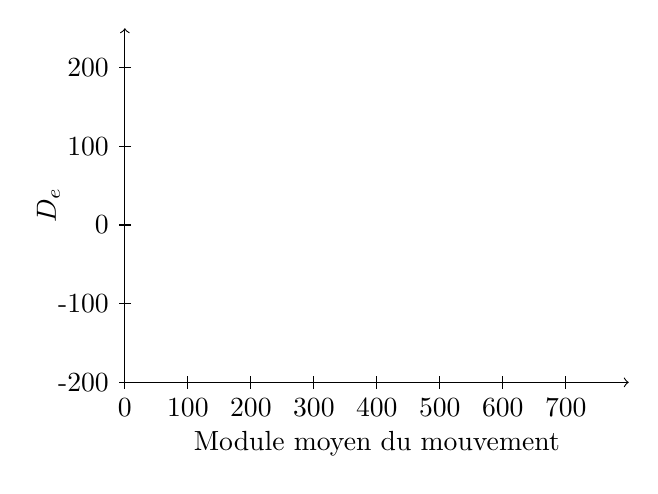
\begin{tikzpicture}[only marks, xscale=0.08, yscale=0.01]
	\pgfsetplotmarksize{1cm}
	\draw plot[mark=+,mark options={yscale=8}] file {plot/chap7/MV-erreurDMOS.txt};
	\draw[->] (0,-200) -- node[below=0.5cm] {Module moyen du mouvement} coordinate (x axis) (80,-200);
	\draw[->] (0,-200) -- node[rotate=90, above=0.7cm] {$D_e$} coordinate (y axis) (0,250);
	\draw (0, -192) -- (0,-208) node[anchor=north] {0};
	\draw (10, -192) -- (10,-208) node[anchor=north] {100};
	\draw (20, -192) -- (20,-208) node[anchor=north] {200};
	\draw (30, -192) -- (30,-208) node[anchor=north] {300};
	\draw (40, -192) -- (40,-208) node[anchor=north] {400};
	\draw (50, -192) -- (50,-208) node[anchor=north] {500};
	\draw (60, -192) -- (60,-208) node[anchor=north] {600};
	\draw (70, -192) -- (70,-208) node[anchor=north] {700};
	\foreach \y in {-200,-100,0,100,200} \draw (1,\y) -- (-1,\y) node[anchor=east] {\y};
	\end{tikzpicture}
	\caption{Différence d'erreur de prédiction entre VQM et notre critère utilisant des tubes spatio-temporels en fonction du module moyen du mouvement pour les 42 séquences de la base d'évaluation.}
	\label{fig:MV-erreurDMOS}
\end{figure}


\subsection{Discussion}
\subsubsection{Sur la méthode}
Nous avons utilisé ici la même méthode de segmentation spatio-temporelle qu'au chapitre précédent, celle présentée au chapitre~\ref{chap:methode}. Elle nous fournit les vecteurs de mouvement des tubes spatio-temporels, ce qui permet de construire les tubes et d'y calculer les caractéristiques primaires. Dans le chapitre précédent, seules les proportions étaient exploitées, ce qui permettait d'envisager une méthode d'obtention différente, et notamment plus rapide. Ici, nous avons besoin d'effectuer toute l'estimation de mouvement, ce qui nécessite beaucoup plus de ressources calculatoires. De plus, la transformation en luminances perceptuelles puis l'extraction des caractéristiques primaires sont des traitements couteux en nombre d'opérations, qui laissent plus difficilement envisager la possibilité d'obtenir un critère de ce type produisant un résultat en temps-réel.

Le grand avantage de ce critère sur celui présenté au chapitre précédent est qu'il n'est pas lié au codage. En effet, il n'utilise pas le débit de codage comme paramètre. Ainsi, il pourrait être adapté à des contextes différents de celui de l'estimation de qualité de séquences codées. Il pourrait alors être intéressant d'utiliser des caractéristiques primaires plus adaptées à ces contextes.

% Au final, ce critère forme un compromis intéressant. D'un côté, il prend en compte certains phénomènes complexes que nous avons décrits auparavant comme la transformation en luminances perceptuelles ou les cumuls temporels élaborés. D'un autre côté, il utilise des méthodes simples mais efficaces d'obtention de résultats intermédiaires comme le calcul de caractéristiques ou le calcul de différence.


\subsubsection{Sur les performances}
Aucune des différences entre indicateurs de performance obtenus par les trois critères n'est statistiquement significative. Cela n'est pas très surprenant, étant donné le faible nombre de séquences utilisées. Néanmoins, l'écart avec VSSIM est assez important et confirme les performances plus réduites de ce critère dans un contexte de vidéo haute définition. Par contre, l'écart de performances avec VQM est plus restreint, mais tous les indicateurs s'accordent sur une supériorité sensible de notre critère.

L'objectif était également de montrer dans quelle mesure la prise en compte du mouvement était intéressante dans la construction des tubes spatio-temporels. En comparant les deux ensembles d'indicateurs obtenus, il est clair que cette approche apporte un gain sensible. D'ailleurs, il est intéressant de remarquer que les indicateurs obtenus par notre critère utilisé avec des tubes fixes et ceux obtenus par VQM sont quasiment identiques. Ainsi, le gain en performances obtenu par notre approche par tubes orientés selon le mouvement est du même niveau que celui entre VQM et notre meilleur critère. Une analyse par contenu ne nous a cependant pas permis pour l'instant de relier les différence de prédiction aux caractéristiques des séquences.

Pour distinguer les trois critères en termes de complexité calculatoire, le tableau~\ref{tab:diffVQM3DFixes} présente leurs principaux éléments de complexité. VQM débute son traitement par une étape de calibrage que notre approche n'utilise pas. Cela permet à VQM d'être insensible aux décalages spatiaux et temporels de l'image et aux changements de contraste et de luminance entre la séquence de référence et la séquence dégradée. C'est un avantage dans le cas où ce type de phénomènes se produit comme par exemple en présence d'erreurs de transmission, ce qui n'est pas notre cas. De plus, VQM utilise une combinaison de plusieurs paramètres de qualité. Trois cumuls, qui peuvent être différents pour chaque paramètre, sont ensuite effectués. Tout ceci conduit à une plus grande complexité de VQM par rapport à notre critère utilisant des tubes fixes, alors que les performances sont identiques. En revanche, notre meilleur critère utilise une estimation de mouvement. Cette étape seule entraine d'une part une augmentation importante de la complexité du critère, mais permet un gain significatif de performances vis-à-vis de VQM et du critère utilisant des tubes fixes.

\begin{table}[htbp]
\centering
\begin{tabular}{cccc}\toprule
\multirow{2}{4cm}{\textbf{éléments de complexité}}	& \multirow{2}{2.5cm}{\strong{VQM modèle \emph{Television}}}	& \multicolumn{2}{c}{\strong{notre approche}}	\\ \cmidrule{3-4}
												& 				& \textbf{tubes 2D + t}				& \textbf{tubes 2D + M$^\text{t}$}					\\ \toprule
calibrage									& oui 															& non								& non							\\ \midrule
estimation de mouvement		& non															& non								& oui 							\\ \midrule
caractéristiques primaires		& 4																& 1									& 1	 							\\ \midrule
paramètres de qualité 			& 2																& 1									& 1	 							\\ \midrule
cumul spatial							& 6																& 1									& 1								\\ \midrule
cumul temporel						& 7																& 1									& 1								\\ \midrule
cumul inter-caractéristique		& 1																& 0									& 0								\\ \bottomrule
\end{tabular}
\caption{Principaux éléments de complexité du critère VQM et de nos deux critères.}
\label{tab:diffVQM3DFixes}
\end{table}


\subsection{Conclusion}
Dans cette section, nous avons conçu, développé et évalué un second critère objectif de qualité vidéo avec référence complète basé sur le calcul de caractéristiques dans des éléments spatio-temporels élémentaires. Pour cela, nous nous sommes appuyés sur la méthode de segmentation spatio-temporelle présentée au chapitre~\ref{chap:methode}. Des caractéristiques primaires, calculées respectivement dans les tubes des séquences de référence et dans les tubes des séquences dégradées, sont ensuite comparées afin de mesurer l'impact des distorsions sur la qualité des séquences dégradées. Un cumul temporel est assuré par des fonctions élaborées modélisant d'une certaine façon le processus d'intégration temporelle du système visuel humain. Il fournit la note finale de qualité.


\section{Conclusion}
Dans ce chapitre, nous avons proposé deux approches différentes d'exploitation des résultats de la segmentation spatio-temporelle présentée précédemment (chapitre~\ref{chap:methode}) dans un critère objectif de qualité visuelle. La première approche est basée sur la construction des fonctions de gêne locales et l'intégration des pertes de qualité qu'elles fournissent par les fonctions de cumul présentées section~\ref{sec:deLocalAGlobal}. Bien que la fonction de gêne des zones homogènes de faible luminance soit très performante dans sa prédiction des pertes locales, les autres fonctions ne réussissent pas à fournir des performantes suffisantes. Ainsi, le critère final n'obtient au mieux qu'un coefficient de corrélation de 0,6427 et une racine carrée de l'erreur quadratique moyenne de 14,2177. L'une des raisons pour expliquer ces performances insuffisantes est le manque d'apprentissage des différentes fonctions de gêne, due au nombre restreint de notes subjectives disponibles. %Le cumul qui suit ne permet pas de rattraper les défauts individuels des fonctions de gêne.

La deuxième approche est basée sur l'exploitation des tubes spatio-temporels. Nous avons cherché principalement à valider l'intérêt de prendre en compte le mouvement local dans la construction des tubes. Les performances obtenues par ce second critère de qualité montrent à la fois un gain par rapport au même critère n'utilisant pas le mouvement (tubes fixes), mais également par rapport aux critères VQM et VSSIM. En effet, ce second critère avec prise en compte du mouvement local produit de bonnes performances. Alors que le coefficient de corrélation entre les qualités prédites et les qualités mesurées est de 0,8749 pour VQM et 0,8368 pour VSSIM, ce second critère permet d'atteindre 0,8977. La racine carrée de l'erreur quadratique moyenne est respectivement de 8,3049, 8,9829 et de 10,1524 pour notre critère, VQM et VSSIM. Ces indicateurs de performance montrent la légère supériorité de notre critère. Aucune des différences entre indicateurs n'est cependant significative sur une base d'évaluation de 42 séquences. L'intérêt principal du critère est plus évident lorsqu'il est utilisé avec des tubes fixes au cours du temps. En effet, le coefficient de corrélation obtenu dans ce cas est de 0,8748 et la racine carrée de l'erreur quadratique moyenne est de 9,0807 dans les meilleures conditions. Pour une complexité moindre, cette version du critère obtient des performances similaires à VQM. C'est donc au prix d'une complexité accrue due à l'estimation de mouvement, que l'adaptation des tubes au mouvement local permet un gain sensible en performances.

\ornementChapitre
